% Template by - Santiago Morante
% Slightly modified by - David Estevez

\documentclass[11pt,a4paper,twoside]{book}
\usepackage{authoraftertitle}
\usepackage[pdftex]{hyperref}
\usepackage{graphicx}
\usepackage[english]{babel}
\usepackage[utf8]{inputenc}
\usepackage{fancyhdr}
\usepackage{invuc3mlib}
\usepackage{url}
\usepackage{apacite}
\usepackage[nottoc,notlof,notlot]{tocbibind}%was commented out.
\usepackage{palatino}
\usepackage[Lenny]{fncychap}
\usepackage[font=small,format=plain,labelfont=bf,up,textfont=it,up]{caption}
\usepackage{colortbl}
\usepackage{indentfirst}
\usepackage{hhline}
\usepackage{mathtools}
\usepackage{amsmath}
\usepackage{amsfonts}
\hypersetup{  
    pdftitle={Master Thesis - David Estevez Fernandez},
    pdfsubject={Master Thesis - David Estevez Fernandez},
    pdfauthor={David Estevez Fernandez},
    pdfkeywords={clothes} {folding},
    colorlinks,
    citecolor=black,
    filecolor=black,
    linkcolor=black,
    urlcolor=black, } 

\usepackage[twoside]{geometry}
\geometry{twoside, bindingoffset=1cm, papersize={210mm,297mm}, total ={135mm, 220mm}, includefoot, includehead}

\setlength{\topmargin}{0cm} 
\setlength{\headsep}{8mm}
\setlength{\marginparwidth}{20mm} \setlength{\evensidemargin}{4mm} \setlength{\oddsidemargin}{20mm}
\newcommand{\clearemptydoublepage}{\newpage{\pagestyle{empty}%
\cleardoublepage}}

% Define a command for comments
\usepackage{color}
\newcommand{\comment}[1]{\textbf{\color{cyan} #1}}
\newcommand{\warning}[1]{\textbf{\color{red} #1}}
\newcommand{\reftodo}[0]{\textbf{\color{magenta} [Ref]~}}

% Non-standard comments (require package latex-xcolor)
\usepackage[dvipsnames]{xcolor}
\newcommand{\juansays}[1]{\textit{\color{Plum} #1}}

\usepackage[english]{babel}

% Imports for images
\usepackage{caption}
\usepackage{subcaption}
\usepackage{wrapfig}

% Fix ugly urls
\newcommand{\stdurl}[1] { \urlstyle{same}\url{#1} }

% Cool large table variables
\newcommand{\bigtablewidth}{0.49\textwidth}

% Name of each result category
\newcommand{\fail}{Bad}
\newcommand{\good}{Fair}
\newcommand{\great}{Good}
\newcommand{\discarded}{Discarded}

\begin{document}
	\title{\textbf{Towards Robotic Clothes Folding:\\A Garment-Agnostic Unfolding Algorithm}}
	\author{David Estevez Fernandez}
	\tutor{Juan G. Victores}
  	\stutor{Carlos Balaguer}

        \primerjurado{Dr./Dra.}
        \segundojurado{Dr./Dra.}
        \thirdreader{Dr./Dra.}
		
    \dedicate{
		\begin{flushright}
   		\warning{``It's better to have loved and lost than to have to do forty pounds of laundry a week.''\\    
    Laurence J. Peter}
		\end{flushright}
    }

    \beforepreface

    \prefacesection{Acknowledgments}
   Thanks to all ...
   
   \warning{Thanks to the anonymous donor of the lost red sweater, which was very useful in testing and debugging the algorithms of this work.}

  	\prefacesection{Resumen}
   	 
Esta tesis desarrolla ...

		\prefacesection{Abstract}
This thesis develops ...

	\cleardoublepage
    	\afterpreface

	\pagestyle{fancyplain}
	\renewcommand{\chaptermark}[1] %
	{\markboth{#1}{\thechapter\ #1}}
	\renewcommand{\sectionmark}[1]%
	{\markright{\thesection\ #1}}
	\lhead[\fancyplain{}{\bfseries\thepage}]
	{\fancyplain{}{\bfseries\rightmark}}
	\rhead[\fancyplain{}{\bfseries\leftmark}] {\fancyplain{}{\bfseries\thepage}}
	\cfoot{}
	
	\chapter{Introduction}
\label{introduction}

Folding clothes is a common and necessary, but tedious, task for humans. Additionally, due to the increasing aging of the world population, a growing need exists for automated solutions to be able to help us with laundry. The textile industry another current source of demand for automated solutions. Current industrial solutions, shown in Figure \ref{fig:current_solutions} include human workers and voluminous machines. These machines are bulky, expensive, and require a large dedicated space, as they are intented to be used in an industrial environment. In addition, due to the complexity of garment manipulation tasks, these solutions are designed to be integrated into  assembly lines, with several machines coupled to perform the whole process. Therefore, they are not suitable for domestic use. The proposed alternative is to use a robot to perform these garment manipulation tasks. A humanoid robot, designed to work in human environments, and to have human-like locomotion and manipulation capabilities seems to be a sensible choice.

\begin{figure}[htbp]
		\centering
        \begin{subfigure}[l]{0.42\textwidth}
            \centering
    		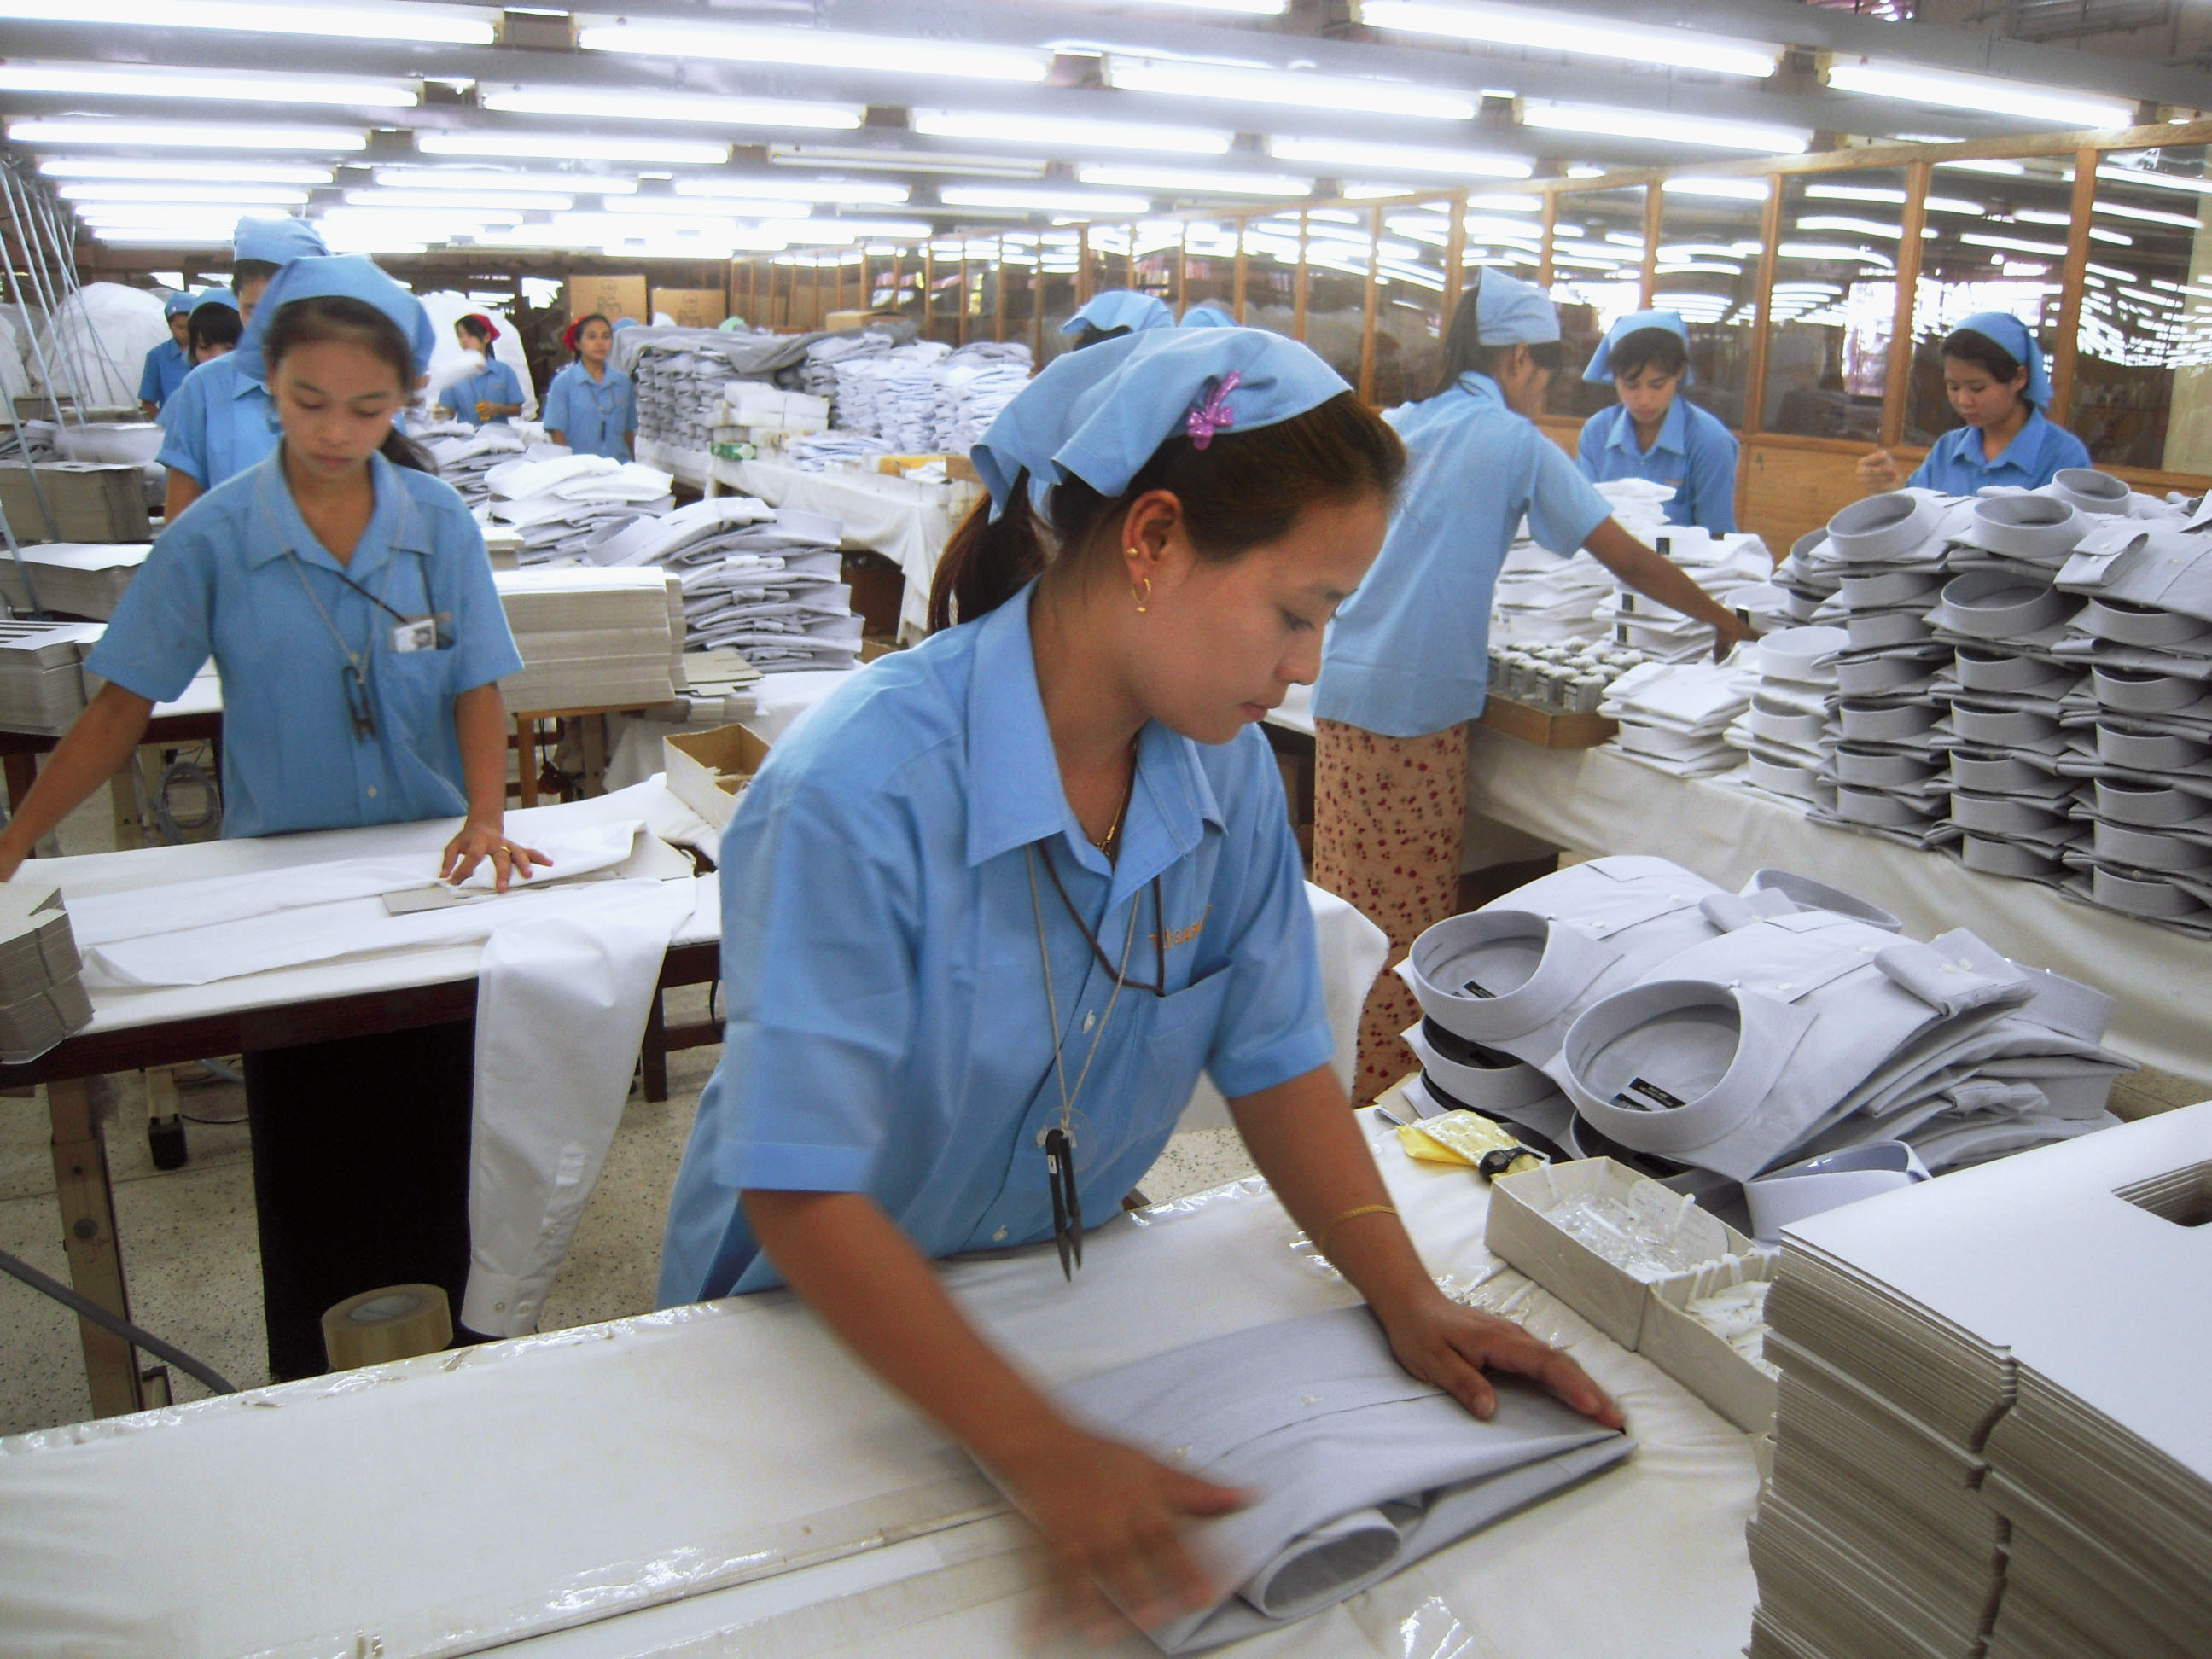
\includegraphics[width=\textwidth]
    		{figures/Intro_japan_folding.jpg}
			\caption{Human-based folding} %http://www.japantimes.co.jp/news/2012/12/19/reference/firms-move-some-eggs-out-of-china-basket/
        \end{subfigure}
        ~
        \begin{subfigure}[r]{0.56\textwidth}
	        \centering
    		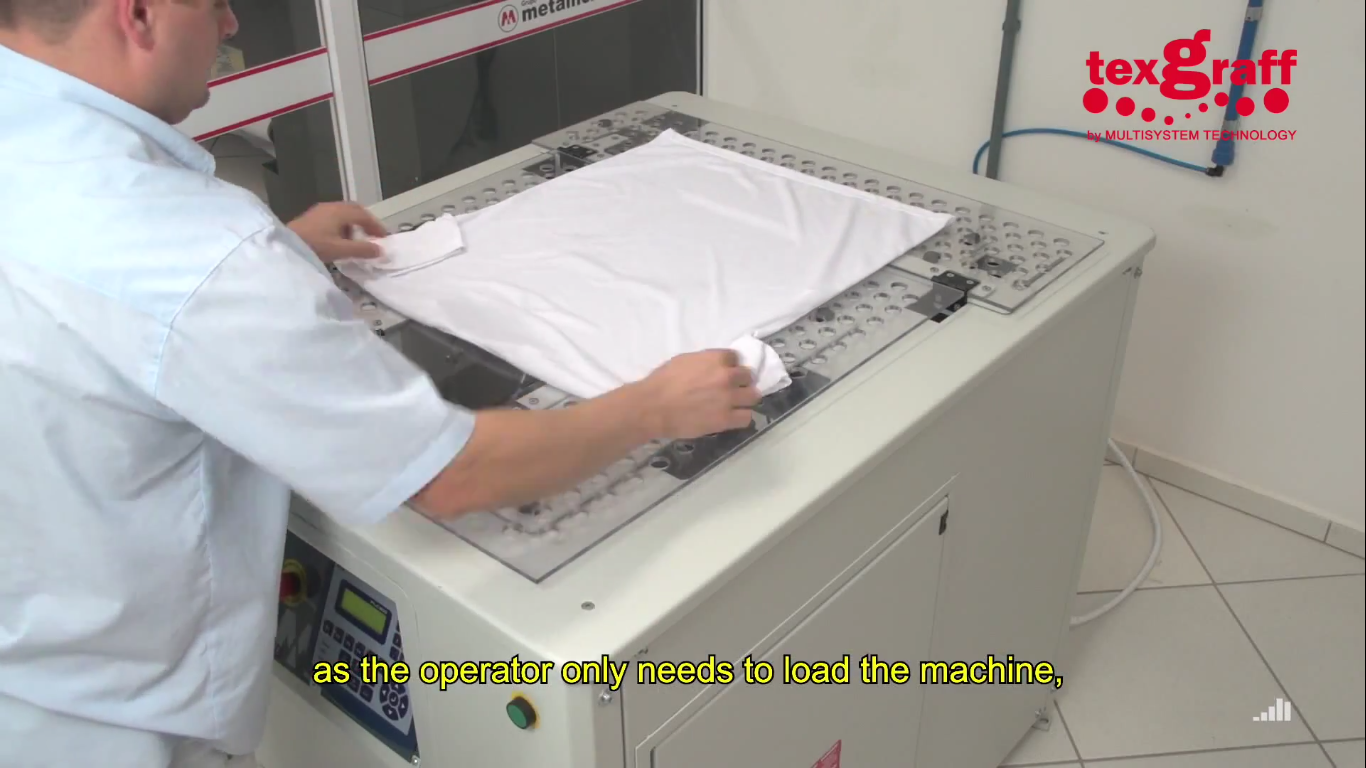
\includegraphics[width=\textwidth]
    		{figures/Intro_industrial_folding.png}
		    \caption{Automatic folding}        
		\end{subfigure} 
		\caption[Current clothes folding solutions available for garment folding]{Current clothes folding solutions available for garment folding. On the left, human workers folding clothes in a textile factory\footnotemark. On the right, an automated solution available in the market, manufactured by Texgraff\textcopyright.}
		\label{fig:current_solutions}
\end{figure}



Working with non-rigid objects such as clothes is a difficult task for robots, due to the complexity of modeling and manipulating deformable, thin objects. Clothes can be easily entangled when doing laundry, and recognizing individual garments and their category just from color or depth image analysis becomes an almost impossible task, due to occlusions amongst the cluttered clothes. Another challenging aspect when working with deformable objects is how to bring the object into a known configuration from an arbitrary initial state.

\footnotetext{Source:\\stdurl{http://www.japantimes.co.jp/news/2012/12/19/reference/firms-move-some-eggs-out-of-china-basket/}}

Extensive work can be found in literature about automated clothes folding once the garment category has been identified (that will be covered in the next chapter), as well as for modeling the garment for fold/wrinkle removal or selecting the most suitable grasping point/strategy. For that reason, this thesis focuses on how to unfold a clothing article that has been picked up from a pile of clothes and is placed on a flat surface. From that point, any of the existing approaches can be applied to fold the garment.

In this thesis the author presents a model-free garment-agnostic algorithm that can compute the pick and place points for a manipulator robot to iteratively unfold a garment, so that other algorithms can then determine the garment category and apply the folding sequence. 

\pagebreak
%This algorithm presents the following advantages:
%
%\begin{itemize}
%\item It provides a general method for detecting folds in
%deformable objects without a prior model of the garment
%to be unfolded.
%\item It computes the best position of the pick point, direction
%of movement, and place point in order to unfold the
%detected fold.
%\item As it uses depth data, it is independent of the color or
%patterns present in the garment, except for background
%extraction
%
%\end{itemize}

It is assumed that a clothing article has already been separated from the rest of the clothes to be folded, and placed on a flat surface. The garment could have been placed on that surface either by a robot or by a human coworker, allowing a collaborative folding pipeline in which a human and a robot can perform different parts of the folding process.
As the algorithm is not based on a geometrical model of the garment to be unfolded, it is general enough to be used with any category of garment, from towels and blankets to trousers or shirts, and with any number of folds. 
%
The presented approach consists in using a depth image from a single point of view to find regions of the garment overlapping other regions, which are considered to be folds. Then, all the possible candidate paths are studied to determine the unfolding direction. This is an iterative process to be repeated until the garment is fully unfolded.

\section{Objectives}
\label{intro_objectives}
The main objective pursued in this work is to develop an algorithm that can estimate the grasping and release points for a deformable object so that a manipulator robot can iteratively unfold a garment. Once unfolded, its garment category  and the folding sequence to apply can both be determined. From the aforehead mentioned algorithm we can deduce the following specific objectives:

\begin{itemize}
	\item It should rely as little as possible in color or patterns present in the garment. This way, the algorithm is more robust and independent from the illumination conditions.
	\item It should provide a general method of detecting folds in deformable objects without a prior model of the garment to be unfolded. The absence of a prior model allows the algorithm to work with any kind of textile article, much as humans work with deformable objects.
	\item It should be able to estimate the best position of the grasping point, direction of movement, and release point in order to unfold the detected fold. An incorrect pick and place sequence would cause the garment to be more entangled that in the initial state, making the unfolding task even more complicated.
\end{itemize}


This work will aim to accomplish these specific objectives in order to solve the presented main objective of garment unfolding.

\section{Document Structure}
\label{intro_structure}

This section presents an overview of the concepts and contents contained in each of the chapters of this thesis. This way, the reader may consume this work in a linear fashion, from start to end, or concentrate on specific parts that are relevant to him. For that purpose the author has tried, whenever possible, to write chapters as much self-contained as possible.

\begin{itemize}
\item \textbf{Chapter \ref{state_of_the_art}} provides an overview of the current state of the different methods and techniques to achieve automatic robot garment folding. It includes techniques based both on modeling and manipulation, as well as works performed as part of the CloPeMa FP7 European project. This chapter is recommended to obtain a general knowledge of other existing approaches that address the same challenges as this work.
\item \textbf{Chapter \ref{architecture}} is related to the actual algorithm developed in this work. This chapter provides a general knowledge of the algorithm and its several stages, and therefore it is recommended that the reader reviews it to understand each concrete part in posterior chapters.
\item \textbf{Chapter \ref{garment_segmentation}} deals with the different steps that constitute the Garment Segmentation stage. This stage is required to determine which pixels of the input images correspond to the garment and which ones correspond to the background.
\item \textbf{Chapter \ref{garment_clustering}} describes the different steps involved in the Garment Depth Map clustering stage. In this stage the pixels from the input depth image are grouped in regions of similar depth, to determine overlapping parts of the garment.
\item \textbf{Chapter \ref{pick_and_place}} presents the different steps involved in the Garment Pick and Place Points stage, explaining how the different steps in this stage generate pick and place points for the humanoid robot to manipulate the garment.
\item \textbf{Chapter \ref{experiments_and_results}} is related to the different experiments performed to validate the algorithm. This chapter describes the experimental setup as well as the various experiments and results obtained from them.
\item \textbf{Chapter \ref{conclusions_and_future_work}} finally offers an analysis of the work and main contributions. The issues arised during the execution of this work are also mentioned, along with some lines of future work in order to address them.
\end{itemize}

	\chapter{State of the Art}
\label{state_of_the_art}

\comment{Thesifize this}

A significant amount of work conducted in this topic has been focused on modeling the different garment categories for both unfolded, extended garments and for grasped garments. The computer vision community has contributed with extensive work on the specifics of clothes modeling \cite{Chen2009}. 

Kita et al. propose a method that uses a deformable model to calculate the state of hanging clothes based on 3D observed data \cite{Kita2004, Kita2009}. This calculation is performed by generating a set of candidate shapes predicted by physical simulations of hanging clothes and later comparison of them with the observed data. To fit the observed 3D data better, each generated shape is further deformed and the shape that is more consistent with the observed data is selected. 

Miller et al. present an approach to modeling the clothes when already spread out on a flat surface in \cite{Miller2011}. A series of parametrized shape models are proposed, each clothing category having its own model. Garment variability is solved through variation of those parameters. Once the garment has been modeled with their method, a preprogrammed folding sequence can be performed.

A method for classifying and estimating the poses of deformable objects is presented in \cite{Li2014ICRA}. This method consists in creating a training set of deformable objects by off-line simulation of different garments, extracting depth images from different points of view. Then, a codebook is built for a set of different poses of each deformable object by extracting features from the dataset and applying sparse coding and dictionary learning. With this codebook, classifying deformable objects on different categories and estimating their current pose is possible, for later regrasping or folding the garment.

The previous method was improved in \cite{Li2014IROS}, by extracting the features directly from the 3D data, dividing the hanging garment in different cells via layers, rings and sectors of the bounding cylinder. Each of the sectors becomes a binary feature, using the Signed Distance Function to check if the cell is inside the voxel where the center of the cell belongs, and is then arranged in a feature vector. A Hamming distance, whose weights are learned from the simulated dataset merged with some models reconstructed from real word Kinect point clouds, is used to estimate the object category and pose given an input reconstructed mesh model.

Based on the previous recognition algorithm, Li presents in \cite{Li2015ICRA} a method for unfolding deformable objects with a bi-manipulator robot. With this method, the robot is capable of taking a clothing article from an unknown state to a known state by iterative regrasping, detecting the most suitable grasping points in each state to achieve its goal. For locating the most suitable grasping points, the 3D point cloud obtained by the robot is matched to the mesh model, that incorporates the information about the best regions to grasp in order to unfold the garment.

The method introduced by Cusumano-Towner et al. in \cite{Cusumano-Towner2011} allows a bi-manipulator robot to identify a clothing article, estimate its current state and achieve a desired configuration, generalizing to previously unseen garments. For that purpose, the robot uses a Hidden Markov Model (HMM) throughout a sequence of manipulations and observations, in conjunction with a relaxation of a strain-limiting finite element model for cloth simulation that can be solved via convex optimization.

Clothing article manipulation is another field in which extensive work has been done. Osawa et al. propose in \cite{Osawa2006} a method to unfold garments in order to classify them. It consists in alternatively regrasping clothing and expanding them using a two-arms manipulator. The garment is grasped with one arm and the lowest point is located by rotating the piece of clothing, which is used as a grasping point for the other arm. If the garment has any fold when extended, it is placed over a flat surface to repeat this process util the the garment is fully spread out.

To detect the best grasping points for a clothing article, Ramisa \cite{Ramisa2012} performs the identification in a single step, even with highly wrinkled clothes. This detector is based in a Bag of Features detector, using as input a combination of appearance and 3D geometric features.

CloPeMa\footnote{\url{http://www.clopema.eu/}} is a recent EU-FP7 research project (2012-2015) whose objective is to advance the state of the art in perception and manipulation of fabric, textiles and garments. As part of the CloPeMa project, a method to detect single folds has been presented by Mariolis et al. in \cite{Mariolis2013, Mariolis2015}. In order to detect such folds, a database of unfolded clothes templates is built in the first place. These templates are later used to perform a shape matching between the folded garment shape, obtained by the camera, and the unfolded garment model. This process is iterative, and the initial results are feedbacked to adapt the model for a better fit. Stria et al. propose in \cite{Stria2014, Stria2014IROS} a polygon-based model for clothes configuration recognition using the estimated position of the most important landmarks in the clothing article. Once identified, these landmarks can be used for automated folding using a robotic manipulator. The clothes contour is extracted from a RGB image and processed using a modified grabcut algorithm and dynamic programming methods are used to fit it to the polygonal model. Doumanoglou et al. follow in \cite{Doumanoglou2014ECCV} an approach based on Active Random Forests to recognize clothing articles from depth images. This classifier allows the robot to perform actions to collect extra information in order to disambiguate the current hypotheses, such as changing the viewpoint. In \cite{Doumanoglou2014ICRA} they extend this approach to detect the optimal grasping points to unfold the garment.

%\comment{(pseudo-unfolding -> remove wrinkles)}
%\warning{Some work on wrinkles removal has been made by Sun et al. \cite{Sun2015} with a stereo vision system and a dual manipulator robot. Wrinkles are first identified  using a depth map of the cloth, which is later B-spline smoothed and parsed by shape and topology into different wrikle structures, that are later ranked by size and removed.}

The most similar work we can find in the related literature is the method for unfolding clothes presented by Willimon et al. in \cite{Willimon2011}. Their method, which also focuses in clothes unfolding prior to automated folding, use several features obtained from a depth image, such as peak regions and corners location, to determine the location and orientation most suitable for interaction with the garment. Two main steps are performed: first, the clothing article is flattened using RGB information from the camera and, then, depth information is used to extract the features used to estimate how to unfold the garment.
	\chapter{\MyTitle}
\label{architecture}

This chapter presents an overview of a garment-agnostic algorithm to unfold clothes using depth sensor data, that will be extended in later chapters. The pipeline for folding clothes followed throughout robotic literature is based on how it is performed by humans. This allows these tasks to be executed in the same environments as humans, aiming towards a fully-automated or collaborative fashion. Garments are extracted from the washing or drying machine forming a pile, and an iterative process begins. First, an individual clothing article is picked from the pile. Then, the garment is extended in the air or assisted by a flat surface, during which unfolding and wrinkle removing procedures may be performed for aiding the posterior classification and manipulation of the garment. A classification procedure is applied to fit clothing article within a certain garment category. Finally, a standard manipulation sequence specific to its category is applied to fold the garment for storage. This iterative process is repeated until there are no clothes left on the pile.

Our work differs with most of the state of the art in the fact that garment models are not used. Our approach uses depth information captured with an RGB-D sensor to detect folds in a garment. The most suitable grasping position, unfolding direction, and release point are computed.

The algorithm can be divided into three main stages, shown in Figure \ref{fig:pipeline_block_diagram}. First, the  background is extracted from the image and the contour of the garment is approximated. Then, a depth map clustering process is performed to estimate overlapping regions. Finally, the information obtained in the previous process is used to determine if there are any folds present and how to interact with the garment to unfold it. The whole unfolding pipeline is an iterative process, that should be repeated again until the garment is completely extended.

The algorithm has been open sourced and is available online\footnote{\url{https://github.com/roboticslab-uc3m/textiles}}.

\begin{figure}[thpb]
    \centering
    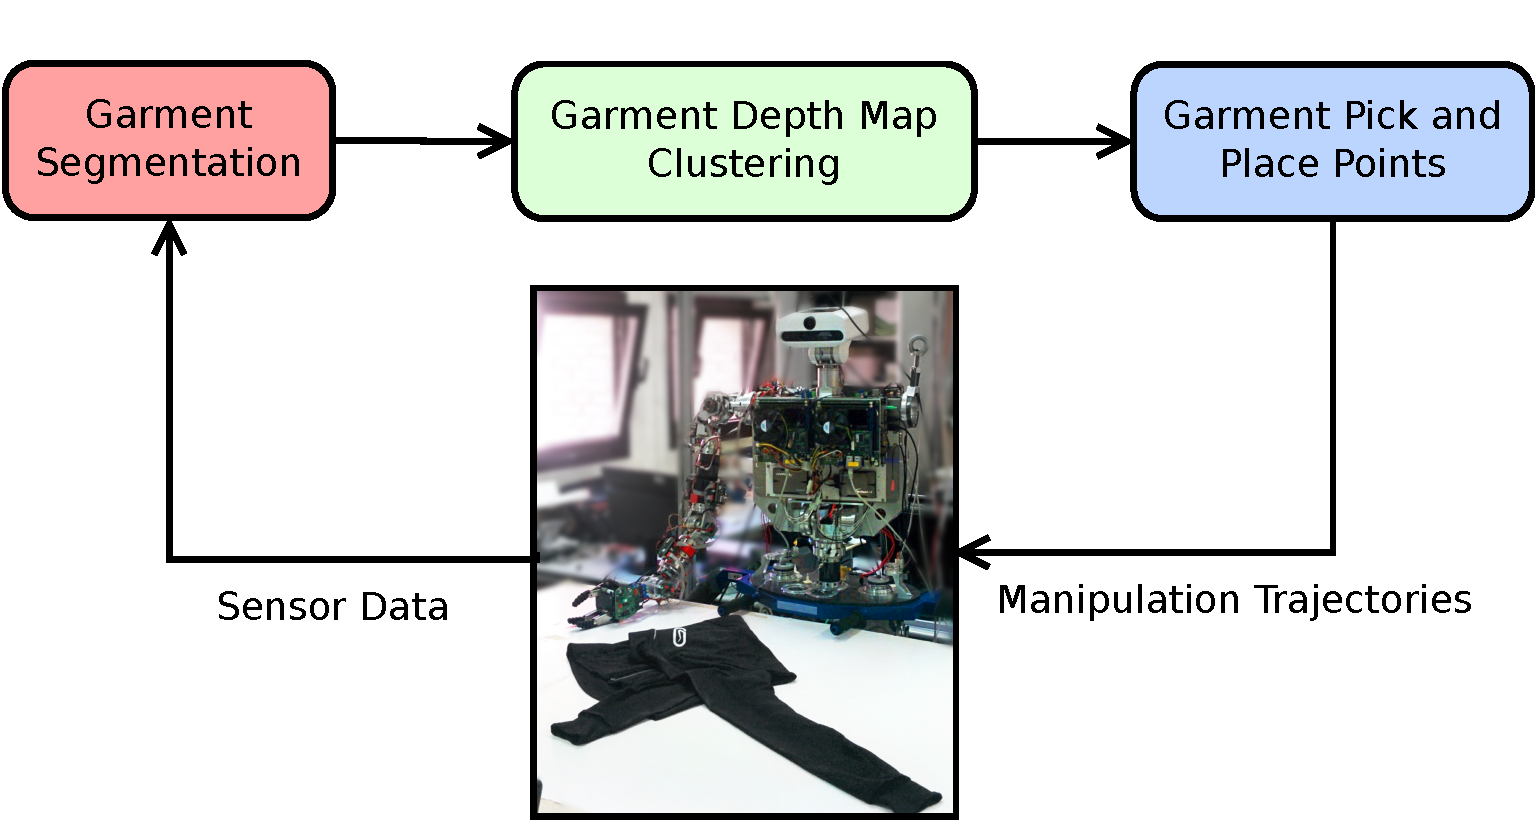
\includegraphics[width=\textwidth]
    {figures/Main_diagram.pdf}
    \caption{Garment Unfolding pipeline. The pipeline uses RGB and depth images captured from the robot sensors as inputs and process them in 3 consecutive stages. This process is iterative, and it is applied until the garment is fully unfolded.}
    \label{fig:pipeline_block_diagram}
\end{figure}

\section{Garment Segmentation}
\label{architecture:garment_segmentation}

The objective of this garment segmentation stage is to substract the background from the input RGB-D image to obtain only the resulting garment data, as well as to extract the simplified garment contour. Figure \ref{fig:generic_garment_segmentation} depicts a generic sample of this background subtraction and contour extraction process.


%\begin{figure}[thpb]
%    \centering
%    
\includegraphics[width=0.8
%    \textwidth]{figures/placeholder2.png}
%    \caption{\comment{A nice figure of a generic Background subtraction and contour extraction}}
%    \label{fig:generic_garment_segmentation}
%\end{figure}


\begin{figure}[htbp]
	\centering
    \begin{subfigure}[l]{0.49\textwidth}
        \centering
    	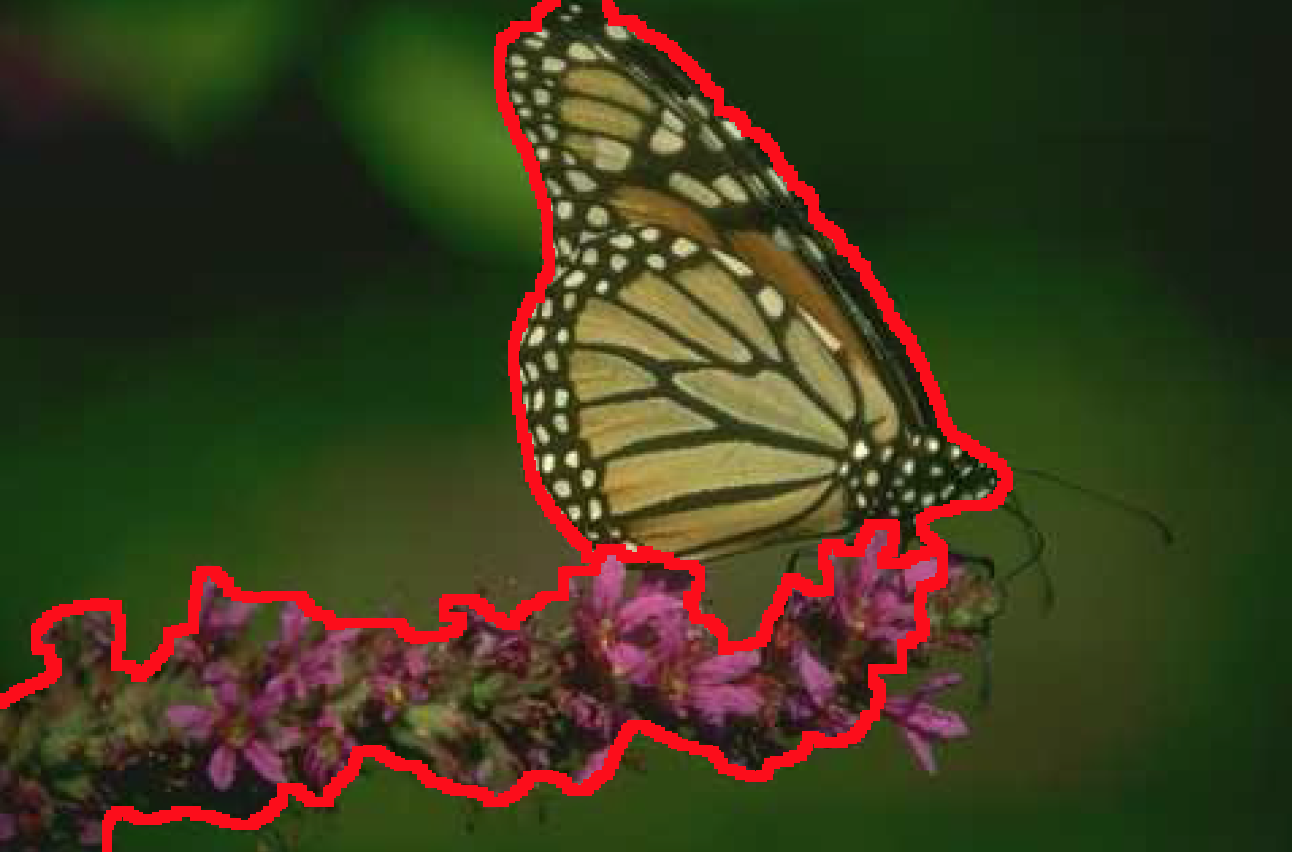
\includegraphics[width=\textwidth]
    	{figures/Background-segmentation-01.png}
        \end{subfigure}
        ~
        \begin{subfigure}[r]{0.49\textwidth}
	        \centering
    		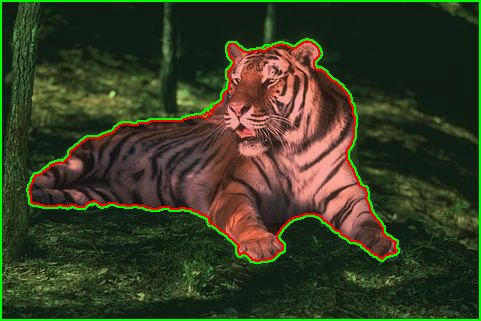
\includegraphics[width=\textwidth]
    		{figures/Background-segmentation-02.jpg}
		\end{subfigure} 
    \caption[dummy]{Two examples of background segmentation. In the left image \cite{ren2013image}, the foreground objects contour is highlighted in red. In the right image\cite{nieuwenhuis-cremers-pami12_2}, the foreground object (the tiger) is highlighted in red, and the background is highlighted in green.}
    \label{fig:generic_garment_segmentation}
\end{figure}


Prior to any further analysis, a background subtraction step has to be performed in order to remove all information not related to the garment. Based on the assumption that the clothing article is placed on top of a flat white surface, the garment can be segmented by color. This can be performed by threshold operations on the red, green and blue channels of the RGB space, or on the hue, saturation and value channels of the HSV space. Other color spaces could also be used. GrabCut \cite{rother2004grabcut}, that uses gaussian mixture models (GMMs) and iterative energy minimization, is another available method to separate the background and foreground based on color.

Another potential approach is to remove the horizontal plane of the table using depth information. This approach can be further improved by combining the results obtained by the depth-based segmentation with a color segmentation, in case the garment color and the background are dissimilar enough.

Once the background is extracted, the contour of the garment has to be determined. Several methods exist for this purpose. The Topological Analysis by Border Following algorithm developed by Suzuki and Abe \cite{suzuki1985topological} is a widely used algorithm for connected-component labeling and countour finding. A Marching Squares algorithm, a variation of the Marching Cubes algorithm \cite{lorensen1987marching}, can be also applied to find constant valued contours in an image.

After the contour is extracted, it is then approximated to a polygon, e.g. using the Ramer-Douglas-Peucker algorithm \cite{ramer1972iterative, douglas1973algorithms}. Alternative algorithms exist, such as the Teh-Chin algorithm to find Dominant Points \cite{teh1989detection}. Each of the segments obtained is a candidate for being a fold axis. The midpoints of those fold axis candidates are calculated to be used in the following steps.

The garment segmentation process used in this thesis is further explained in chapter \ref{garment_segmentation}.

\section{Garment Depth Map Clustering}
\label{architecture:depth_map_clustering}
When the garment has been identified, garment regions with similar height points must be clustered and labeled. By using only depth information, as opposed to using RGB images, makes our algorithm independent of the colors and patterns present in the garments. Many algorithms exist to perform this clustering step.

For general purpose clustering over any set of unlabeled data we can find several algorithms that can be also applied to images. K-means, Mean Shift \cite{comaniciu2002mean} or DBSCAN \cite{ester1996density} are some examples of clustering algorithms that can be applied to group pixels with similar depth.

A particular case of clustering algorithms are those which are applied to obtain superpixels. A superpixel \cite{ren2003learning} is a local region of the image with similar characteristics, such as color, texture, etc. Several examples of superpixel can be seen in Figure \ref{fig:generic_superpixels}. This reduces the number of pixels to regions that are local and coherent, preserving most of the structure of the diferent items at the scale of interest. Many algorithms exist to perform superpixel clustering, such as SLIC \cite{achanta2010slic}, Quickshift \cite{vedaldi2008quick}, Turbopixels \cite{levinshtein2009turbopixels} and Normalized Cuts \cite{mori2005guiding}.

%\begin{figure}[thpb]
%    \centering
%    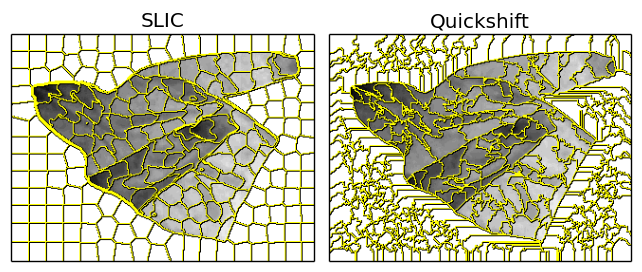
\includegraphics[width=\textwidth]{figures/Superpixels-01.png}
%    \caption{\comment{A nice figure of a generic Superpixels}}
%    \label{fig:generic_superpixels}
%\end{figure}


\begin{figure}[htbp]
	\centering
    \begin{subfigure}[l]{0.51\textwidth}
        \centering
    	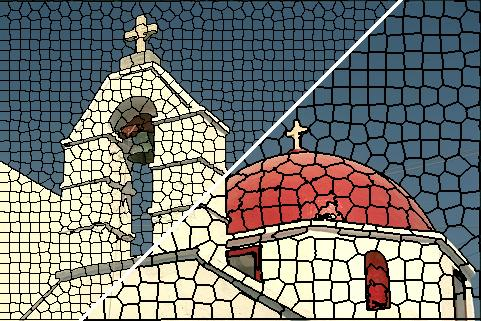
\includegraphics[width=\textwidth]
    	{figures/Superpixels-02.jpg}
    \end{subfigure}
    ~
    \begin{subfigure}[r]{0.47\textwidth}
	    \centering
   		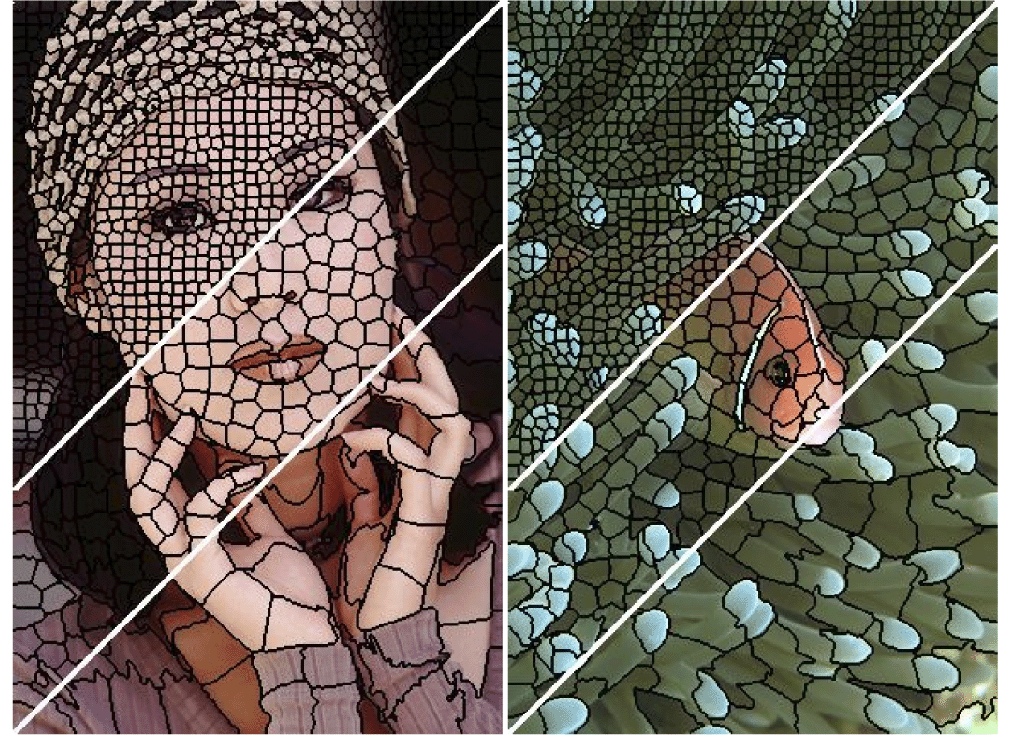
\includegraphics[width=\textwidth]
    	{figures/Superpixels-03.png}
	\end{subfigure}
	\caption[dummy]{Several examples of Superpixel clustering algorithms. Left image \cite{mori2005guiding} corresponds to a Normalized Cut algorithm with two different average cluster sizes, 100 pixels in the case of the upper left part of the image, and 300 in the lower right part. Right image \cite{achanta2012slic}
	 corresponds to a SLIC (Simple Linear Iterative Clustering) algorithm \cite{achanta2010slic} applied to obtain average sizes of 64, 256 and 1024 pixels.}
    \label{fig:generic_superpixels}
\end{figure}

When working with images, the clustering process of finding regions both compact and with homogeneous characteristics is known as segmentation. Many image segmentation algorithms exist based on similar regions and closed contours. One of these algorithms, widely used, is the Watershed transform algorithm \cite{digabel1978iterative}, which interprets the image as a topological surface, filling the image with water from several point sources until they merge, and creating walls in those intersection contours. The regions isolated by these walls are the segmented regions.

The garment depth map clustering process used in this thesis is developed in more detail in chapter \ref{garment_clustering}.

\section{Garment Pick and Place Points}
\label{garment_PnP_points}

Once we have clustered the depth image in regions of similar height, we can proceed to analyze those regions. The objective is to find which parts of the region outline correspond to the fold line, which is physically connected to the rest of the garment. Once the fold line has been detected, pick and place points have to be found for the robot to perform the unfolding operation. Figure \ref{fig:picking_points} displays an example of this unfolding operation, with its pick and place points marked.

\begin{figure}[thpb]
    \centering
    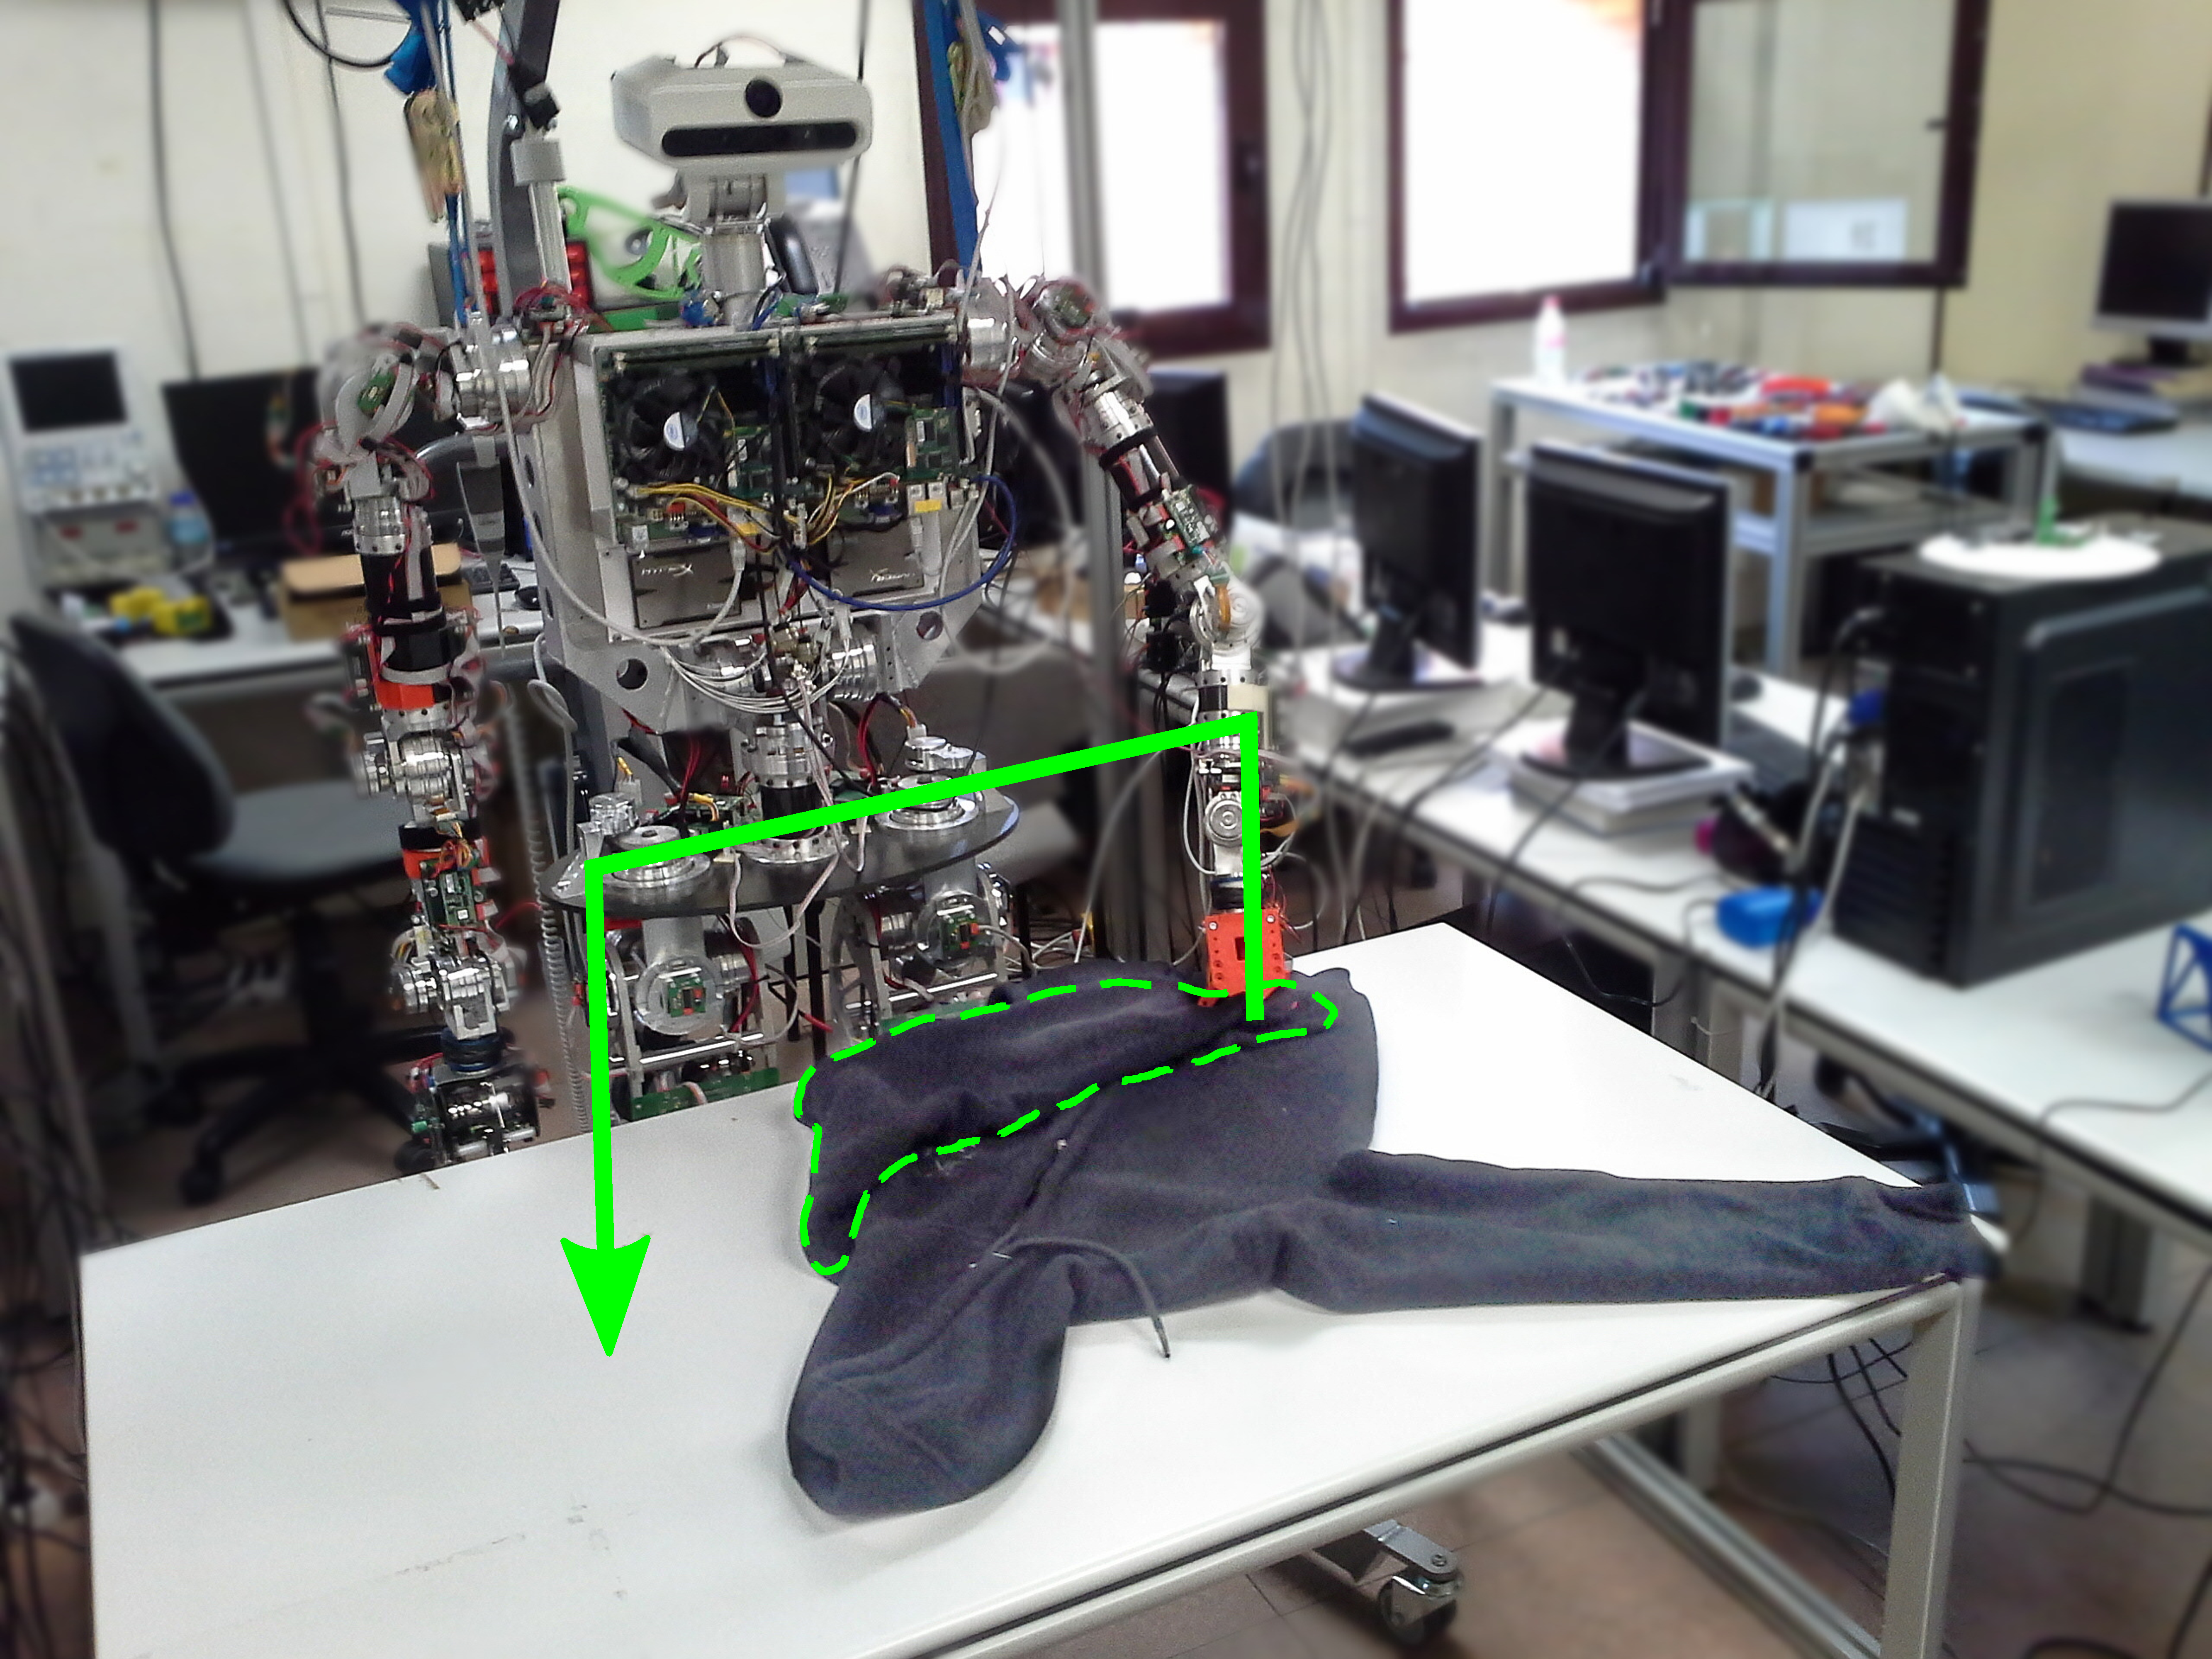
\includegraphics[width=0.8
    \textwidth]{figures/teo-pick-and-place.pdf}
    \caption{An example of an unfolding operation. The figure shows the humanoid robot manipulating a garment. The folded part that is being manipulated, the sleeve, is highlighted with a green dashed line. The green arrow line represents the unfolding trajectory, with the pick and place points at the beginning and the end of it, respectively.}
    \label{fig:picking_points}
\end{figure}


If grouping of certain segmented regions is required, i.e. there are small superpixels with similar characteristics, a merging algorithm has to be performed. A graph-based approach could be used for both merging clusters and determining which clusters are physically connected, either by the fold line or because they belong to the same garment region.


Once the overlapping fold is identified, and the fold line is known, we select pick and place points for performing the unfold operation. This operation, that will be executed by a robot, has to take the garment from the original state to a more ``unfolded'' state.

Several choices exist for pick points, as well as for place points. To pick the garment, one can assume that the highest points in the overlapped region are good candidates, as they probably are easier for the robot to grasp, and they will be separated from the underlying garment. Other potential choices are the points that belong to the border of the overlapping region, except for those which belong to the fold line. These approaches are typically followed by humans when performing unfolding tasks. For place points, the points should be far enough from the garment to completely unfold the overlapping region, but not far enough for the garment to be dragged with the movement. It is also convenient to choose points that lie on the oposite side of the folding line with respect to the pick point, otherwise is almost impossible to perform the unfold operation.
	\chapter{Garment Segmentation}
\label{garment_segmentation}

This chapter is devoted to the first stage of our algorithm, segmenting the garment data from the whole sensor data. The input data is an RGB image with depth information (RGB-D image). Garment segmentation is perfomed over this image, and the garment contour is then extracted and simplified, ready to be used in later stages. \juansays{(Referenciar figura)}

\begin{figure}[thpb]
    \centering
    
\includegraphics[width=0.7
    \textwidth]{figures/placeholder2.png}
    \caption{\comment{(Block diagram for Garment Segmentation chapter)}}
    \label{fig:garment_segmentation_blocks}
\end{figure}


\section{Background Subtraction}
\label{background_subtraction}

The RGB-D image obtained from the robot sensor contains both the clothing article and the table on which it rests. Therefore, after retrieving the data, a background subtraction step is required to classify whether a pixel represents the garment or the table. Figure \ref{fig:background_substration_processes} shows an overview of the different processes involved in this step.


\begin{figure}[thpb]
    \centering
    
\includegraphics[width=0.9
    \textwidth]{figures/placeholder2.png}
    \caption{\comment{Background subtraction processes}}
    \label{fig:background_substration_processes}
\end{figure}

For this purpose, many methods could have been chosen, based on both color and depth information, as discussed in section \ref{architecture:garment_segmentation}. For instance, GrabCut \reftodo was discarded for background subtraction as it requires user input to select background and foreground samples. Furthermore, it is computationally expensive compared with simple thresholding methods. As the main focus of our work is unfolding clothes, a simple color-based method was selected instead. 


We work under the assumption that the garment has been placed over a flat white surface, as opposed to the garment which is much more colorful (higher Saturation). Therefore, the RGB image is converted to the HSV space. Working in the HSV space gives us direct information about our magnitudes of interest: Saturation (S) and Value (V). We are not interested in detecting a particular color, but to detect a colored item, so HSV is a more sensible choice of color space than RGB. 

A filtering process is added to increase robustness and reduce the effect of the noise on the background subtraction. This process is achieved using a convolution with a 5x5 and $\sigma=1.1$ Gaussian kernel computed on the Saturation and Value channels of the HSV image.

Once the image is converted to the HSV color space and filtered, a thresholding operation is then applied to the filtered image, using Otsu's algorithm \reftodo to obtain the optimal threshold values. Pixels with low amount of Saturation, and high Value are classified as being part of the table, as opposed to saturated or dark pixels.

Finally, some morphological transformations are applied to the resulting mask to reduce noise due to false positives/negatives. A 5x5 square kernel is used in several closing operations, followed by a similar number of opening operations. \juansays{"Ya veremos si explicarlo"}

The output of this background substraction step, a binary mask with background pixels represented as black and garment pixels represented as white, can be seen in Figure \ref{fig:segmentation_mask}.

\begin{figure}[thpb]
    \centering
    
\includegraphics[width=0.48
    \textwidth]{figures/placeholder.png}
    \caption{\comment{Again, I should put here a picture of the resulting mask}}
    \label{fig:segmentation_mask}
\end{figure}

\section{Garment Approximated Polygon Computation}
\label{segmentation_approximated_polygon}
From the binary mask obtained in the previous step (section \ref{background_subtraction}) a blob labeling algorithm is applied to detect the garment outline. This outline will be approximated to a simple polygon, and used in later stages to obtain the candidates to be a fold.

\begin{figure}[thpb]
    \centering
    
\includegraphics[width=0.9
    \textwidth]{figures/placeholder2.png}
    \caption{\comment{Garment Polygon calculation processes}}
    \label{fig:garment_polygon_processes}
\end{figure}

The contour extraction method used is the Topological Analysis by Border Following algorithm developed by Suzuki and Abe \reftodo \comment{(suzuki85)}. It was selected as it is a widely used algorithm for connected-component labeling and countour finding. Other algorithms, such as Marching Cubes \reftodo, work under the assumption that contours are isolines\footnote{Curves along which a  function has a constant value.}, which is not the case for binary masks, so they are not suitable. Only external contours are retrieved. A simple chain approximation is then applied to reduce the number of points contained in the contours, storing only the endpoints of the different segments that describe the garment outline.

Due to noise, sometimes some small blobs appear in segmentation masks, so the outline with the largest area is selected as the garment outline. This way, those small blobs are discarded.

After obtaining the garment outline, it is futher processed, as we want to obtain a simplified description of the garment outline. This simplified description is the garment approximated polygon. We assume the fold line has a very high probability of lying in the garment polygon and, therefore, this polygon will represent all the candidate segments to be a fold. To obtain the approximated polygon, the Ramer–Douglas–Peucker algorithm \reftodo is applied. It is selected as it is efficient and a reliable implementation is available in the OpenCV\footnote{http://opencv.org/} libraries used to implement this work. This algorithm recursively divides the outline in segments by choosing the first and last points of the curve and drawing a line. Then, it checks whether that point is closer to that line than a threshold $\epsilon > 0$ or not. If it is closer, all points not marked to be kept can be discarded; otherwise, if it is greater than $\epsilon$, that point is marked to be kept and the procedure is repeated considering the last marked point as ending point. If there are no points left to process, the last point of the outline becomes the ending point again. The previous ending point becomes then the new starting point.

The parameter $\epsilon$ is calculated from the magnitude of the outline perimeter, considering it to be 1\% of that value. The greater this value is, the more simplified the resulting polygon will be.

Figure \ref{fig:contour_and_simplified_contour} shows a comparison between the garment contour, the garment outline and the final approximated polygon.

\begin{figure}[thpb]
    \centering
    
\includegraphics[width=0.9
    \textwidth]{figures/placeholder2.png}
    \caption{\comment{Contour vs outline vs polygon}}
    \label{fig:contour_and_simplified_contour}
\end{figure}

	\chapter{Garment Analysis}
\label{garment_analysis}

This chapter explains in detail the gament analysis that our algorithm performs to the garment data previously segmented. The contour of the garment is extracted, and a Watershed segmentation algorithm is applied to find the different overlapped patches.

\section{Contour extraction}
From the mask obtained in the previous step (section \ref{garment_segmentation_mask}) a blob labeling algorithm is applied to detect the garment outline. This outline will be used in later steps to obtain the candidates to be a fold.

The contour extraction method used is a Topological Analysis by Border Following algorithm developed by Suzuki and Abe\comment{[ref to suzuki85]}. This is a widely used algorithm for connected-component labeling and countour finding. Only external contours were retrieved. A simple chain approximation was then applied to reduce the number of points that describe the contours, storing only the endpoints of the different segments.

Due to noise, sometimes some small blobs appear in segmentation masks, so the extracted contour with the highest area was selected as garment. This way, those small blobs were discarded.

After obtaining the garment contour, it is processed, as we want to obtain a further simplified garment outline. We assume the fold line has a very high probability of lying in the garment outline. Therefore, this contour will represent all the candidate segments that \comment{could be folds.} The Ramer–Douglas–Peucker algorithm \comment{[ref to article]} is applied to obtain the simplified outline. This algorithm recursively divides the contour in segments by choosing the \comment{...}

\section{Watershed segmentation}

Watershed is a segmentation algorithm that considers a greyscale image as a topological surface where high intensity pixels correspond to peaks and hills, and low intensity pixels are equivalent to valleys. The algorithm fills the surface pouring water at each isolated valley. As the water level rises, the water from different sources will start to merge. To prevent them from merging, the algorithm constructs barriers at the merging regions, and continues this process of adding water and building barriers until all the peaks have been flooded. The resulting barriers are the segmentation result, where each region enclosed correspond to a segmented item.

\begin{figure}[thpb]
    \centering
    
\includegraphics[width=0.7
    \textwidth]{figures/placeholder2.png}
    \caption{\comment{(Here it would be great to add a figure of the example, such as opencv's coins)}}
    \label{fig:watershed_example}
\end{figure}


In the context of this work, the Watershed segmentation algorithm is applied to the depth image of the garment to locate the different parts that are overlapping each other. This regions are related to folded parts, that rest on top of other parts of the garment. 

As in practise flooding using local minima as makers leads to over- segmentation, an enhanced version of this algorithm allows the user to specify other criteria for selecting the seed points. The gradient of the greyscale depth-image was calculated for this work, and regions where the gradient has a low value were selected. These regions correspond to homogeneous and continous regions, which are good candidates to be used as markers.

To prepare it for the Watershed segmentation, the depth image was normalized and converted to a greyscale image. A denoising step was also performed, using a total variation filter \comment{(ref chambolle)}, to produce a smoother image, while maintaining the edges sharp. The total variation filter works by minimizing the integral of the norm of the image gradient. As a result of this filter, piecewise-constant images ("cartoon-like" images) are obtained.

The different garment regions obtained with watershed were labeled and used as input for the next step. Figure \ref{fig:watershed_labels} shows the result of this process.

\begin{figure}[thpb]
    \centering
    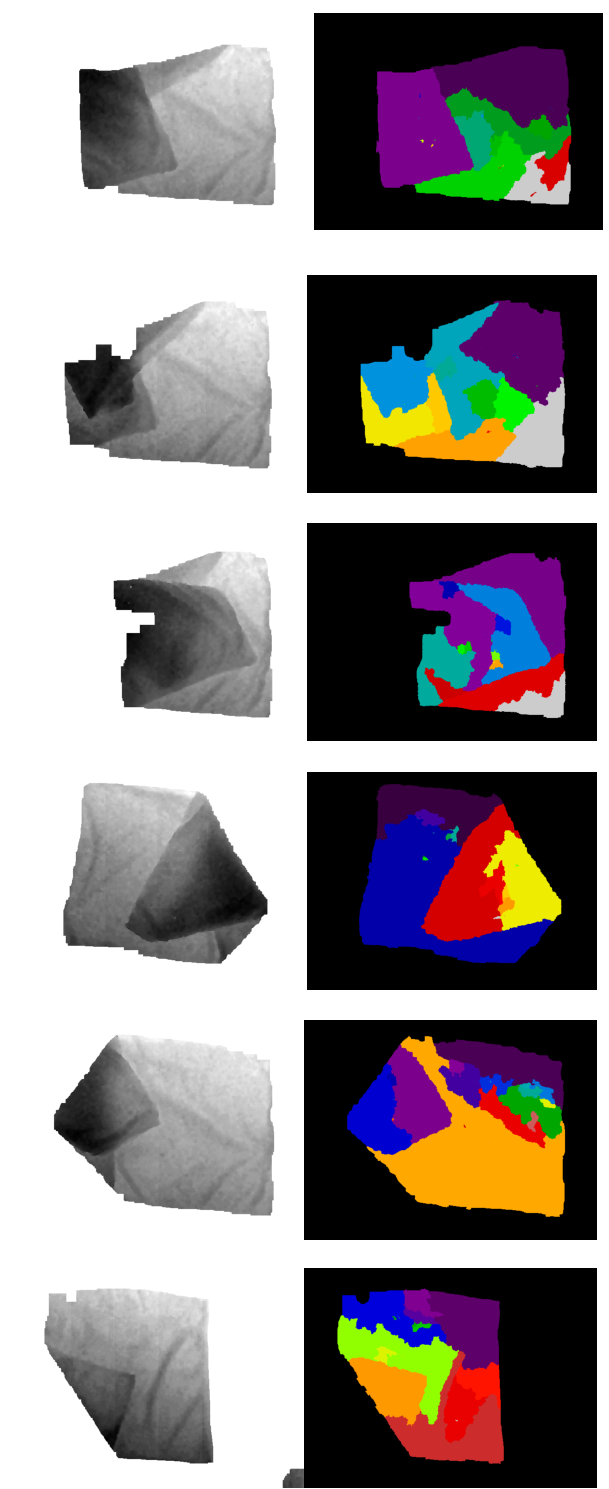
\includegraphics[width=0.38\textwidth]{figures/colour_garment.pdf}
    \caption{On the left side, the grayscale images are shown. The grey level is related to the height of the point as detected by the RGB-D sensor. On the right side, the labeled image returned by watershed algorithm is presented, where each color represents a region of similar height.}
    \label{fig:watershed_labels}
\end{figure}
	\chapter{Garment Pick and Place Points}
\label{pick_and_place}
This chapter explains the last stage of our algorithm, in which the pick and place points required for unfolding the current fold are determined. These points will be later sent to the humanoid robot to perform the unfolding operation. This stage has as input the clustered depth map obtained in the clustering stage (described in chapter \ref{garment_clustering}), and the garment approximated polygon (calculated in section \ref{segmentation_approximated_polygon}). Figure \ref{fig:garment_pnp_points_blocks} shows the block diagram of the different steps that are performed in this stage.

\begin{figure}[thpb]
    \centering
    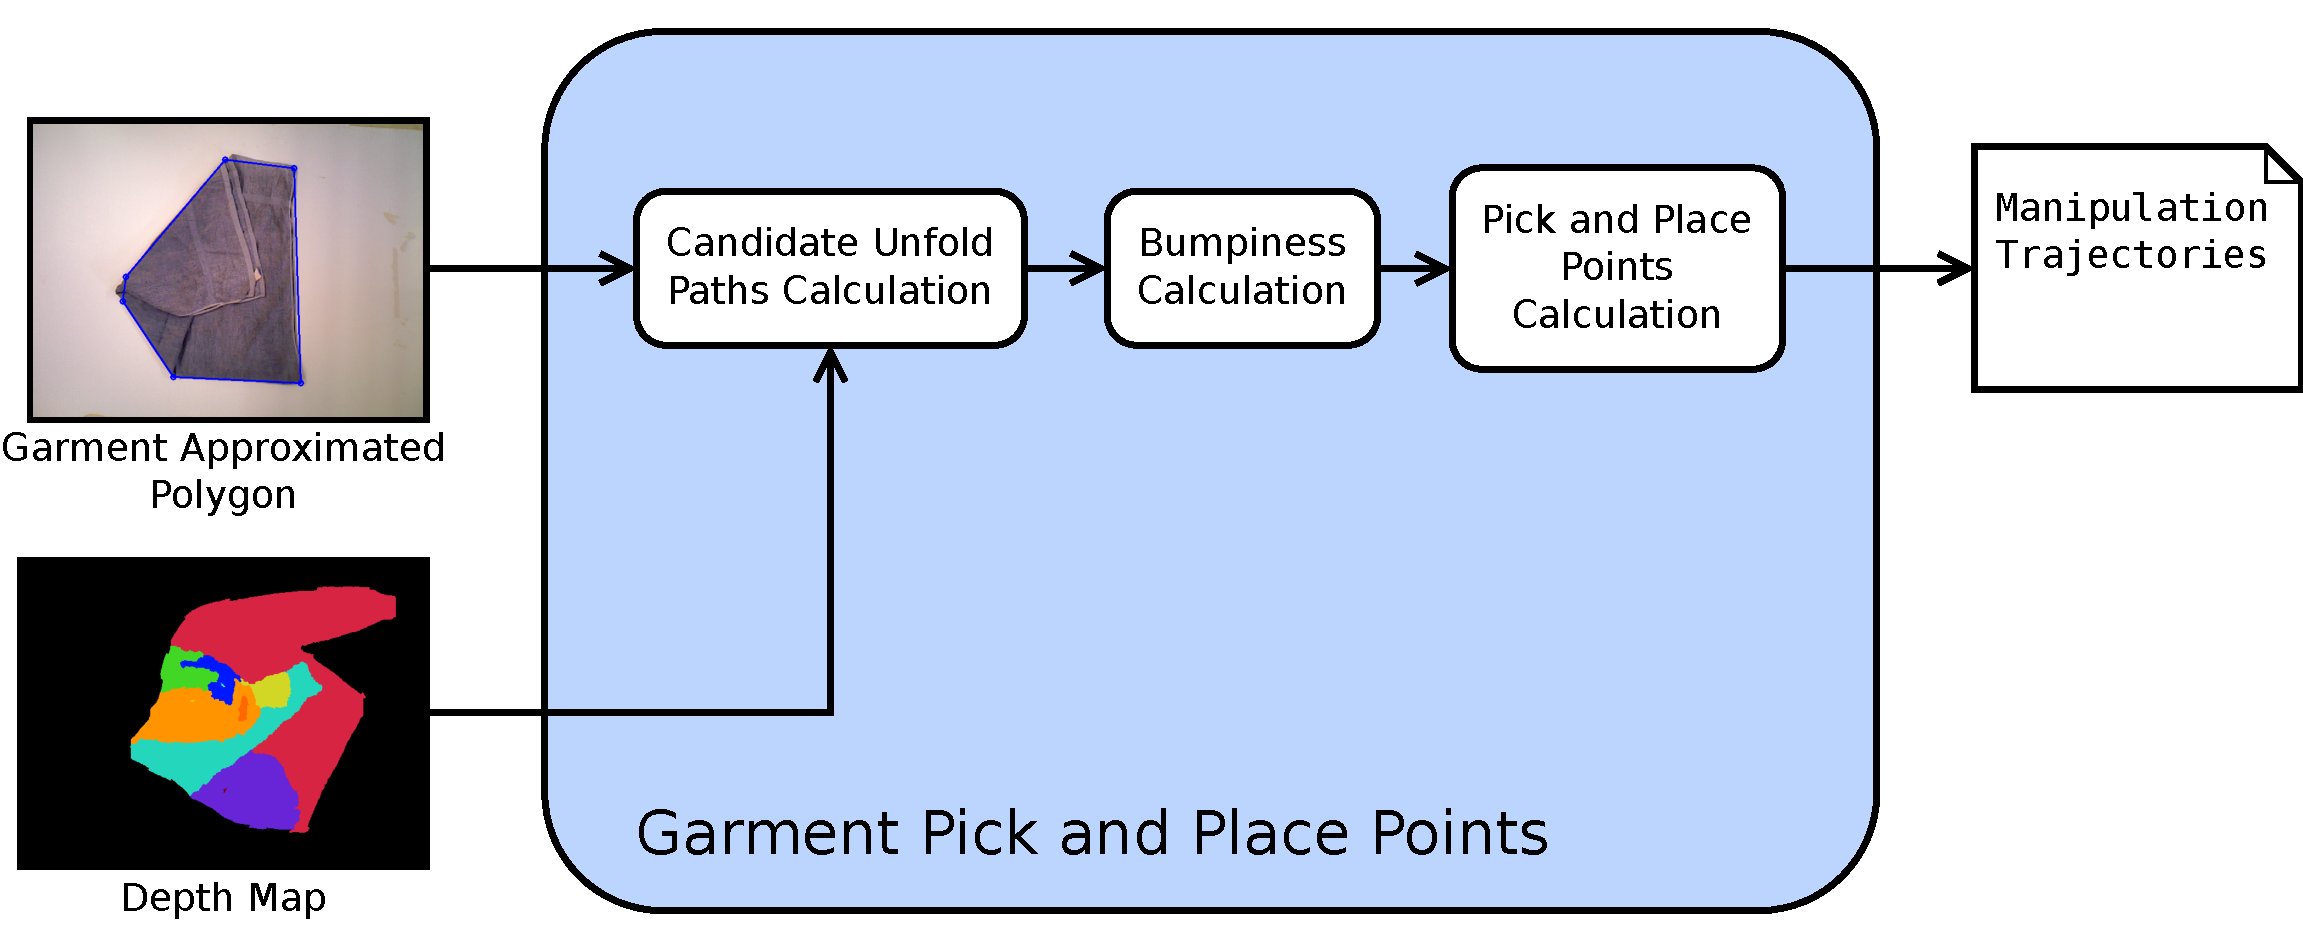
\includegraphics[width=\textwidth]
    {figures/Garment-pnp-points-diagram.pdf}
    \caption{\comment{(Block diagram for Garment Depth Map Clustering chapter)}}
    \label{fig:garment_pnp_points_blocks}
\end{figure}

\section{Candidate Unfold Paths}
\label{unfold_paths}

Based on the assumption that when a garment has an overlapping fold, the fold line will rest on the garment contour, and the folded surface will have lower depth values (i.e. closer to the depth sensor), the next step in our algorithm is to create a set of paths from the highest point of the garment to the midpoint of each contour segment. These paths will be later analyzed using the clusters previously found in the depth image to select the path with less height variation.

To find the highest point in the garment, the clusters previously found with the Watershed algorithm are averaged using the median value for each cluster. Then, the region with the lowest depth value, which is closest to the camera and therefore highest in the garment, is selected as overlapping fold based on the previous assumption. The centroid of the selected cluster is the point selected as the highest point. Using this method instead of selecting directly the highest point from the depth image increases the robustness of the algorithm against outliers and noise present in the depth image.

The midpoint of each segment of the garment approximated polygon is then calculated, and a set of paths departing from the highest point and arriving to the midpoints is created.

These paths are checked so that they are located entirely inside the garment. Paths that go outside the garment approximated polygon are considered invalid. Figure \ref{fig:candidate_paths} shows both the initial paths set and the unfold candidate paths set, without the invalid paths.


\begin{figure}[htbp]
	\centering
    \begin{subfigure}[l]{0.49\textwidth}
	    \centering
    	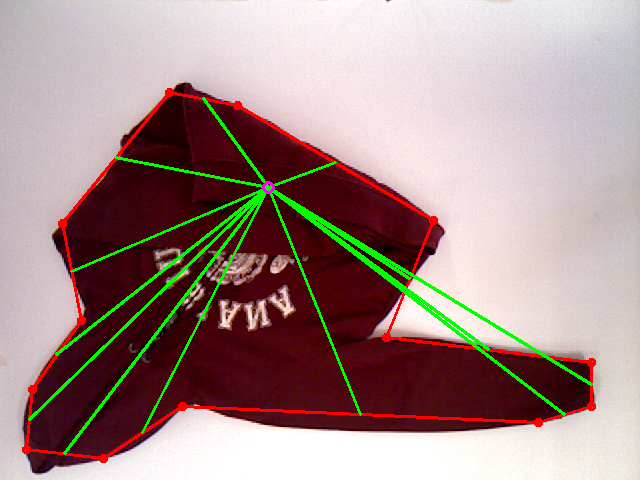
\includegraphics[width=\textwidth]
    	{figures/paths_candidate.png}
    	\caption{Set of candidate paths}
	\end{subfigure}
	~
    \begin{subfigure}[r]{0.49\textwidth}
	    \centering
    	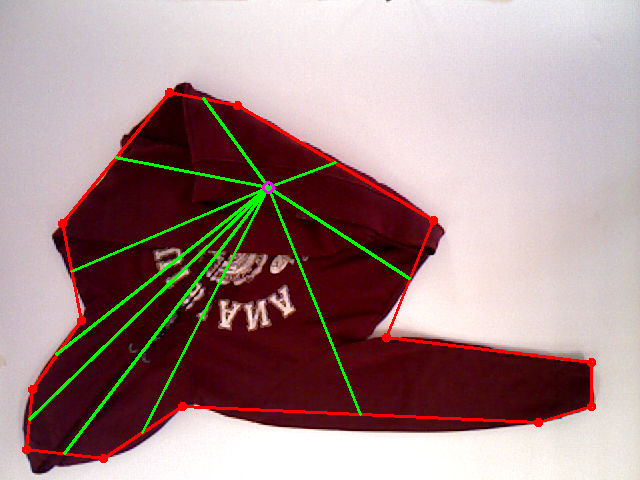
\includegraphics[width=\textwidth]
    	{figures/paths_valid.png}
    	\caption{Set of valid paths}
	\end{subfigure} 
    \caption{\comment{(Figure that shows both the initial path candidate set and the candidate set without the invalid paths)}}
    \label{fig:candidate_paths}
\end{figure}


\section{Bumpiness}
\label{bumpiness}
Each of the candidate paths calculated using the method explained in the previous section has to be analyzed in this step to determine the best unfolding path. 

We can represent each of the $n$ candidate paths obtained as a 2D parametric line ($\mathbb{R} \to \mathbb{R}^2$) depending on a parameter $r$, the radial distance to the highest point:

\begin{equation}
\textrm{path}(r) = \left[u(r), v(r)\right]
\end{equation}

Where $u$ and $v$ are pixel coordinates in the image frame of reference.

Prior to the analysis, each of the paths of length $L$ is discretized in segments with a constant length $l$. The depth image $\mathcal{D}(u,v)$ is sampled at those discrete points. This results in $n$ ordered sets $S=\{ s_1,...,s_m\}$ of depth samples to be analyzed, where:


\begin{equation}
s_i = \mathcal{D}(path(i \cdot l)), \quad  i=0,1,2,..., m
\end{equation}

As the different paths may differ in length $L$, the amount of sampled points ($m=${\Large$\lfloor\frac{L}{l}\rfloor$}) will be different for each path. Figure \ref{fig:paths_with_bumpiness} shows the sample set $S$ corresponding to each candidate path for a certain garment example.

The differences in depth between the overlapping fold region and the rest of the clothing article are assumed to be greater than the diferences in depth within the fold region points. Under that assumption, the metric to evaluate the best path is a \textit{bumpiness} value \textit{B}, which is calculated by penalizing the changes in depth along each of the $n$ candidate sample sets $S$, as shown in Equation \ref{eq:bumpiness}.

\begin{equation}\label{eq:bumpiness}
B = \sum_{i=2}^{m} | s_i- s_{i-1} | 
\end{equation}

The candidate set with the lowest bumpiness value, which corresponds to the path with the least and smallest height changes, is selected as the unfold direction, as shown in Figure \ref{fig:paths_with_bumpiness}.

\begin{figure}[thpb]
    \centering
    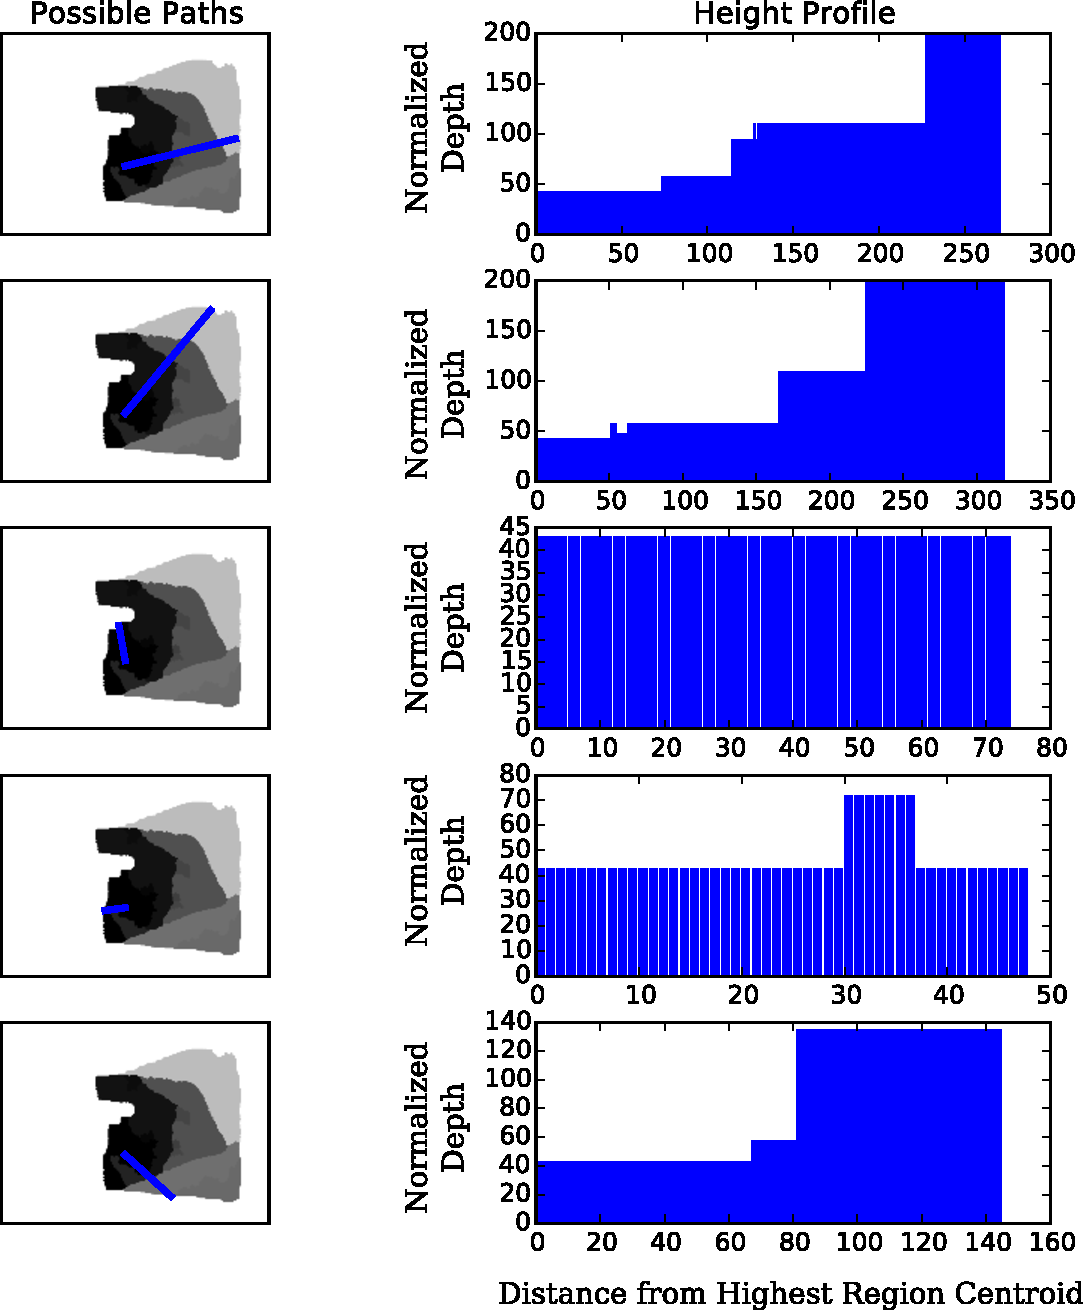
\includegraphics[width=\textwidth]{figures/candidate_paths.pdf}
    \caption{\comment{On the left side, the candidate paths are shown. On the right side, the height profile of each path is shown. Notice that the depth sensor computes the distance to the object from itself, so that a low value in the bar plot means a closer object to the sensor, so it is a region with more height with respect to the table.}}
    \label{fig:paths_with_bumpiness}
\end{figure}

\section{Pick and Place Points}
\label{pick_and_place}
Once the most promising path for unfolding has been identified, the last step is to obtain pick and place points for the robot to perform the unfold action. Due to the absence of a cuantitative metric for determining the suitability of those points, the point selection criteria has been selected using intuition from all possible choices.

The selected grasping point for the picking action is located at the intersection between the unfolding path direction line and the highest garment region border. This point is obtained by calculating the intersection between the selected path line and the highest region contour. This operation results in two intersection points, from which the furthest to the garment border is selected.

The other point is used as axis for a point reflection. To find the placing point, a reflection transformation is applied to the picking point using the aforementioned point as axis. Figure \ref{fig:directions} shows the unfold directions for several clothes, departing at the picking points and arriving to the placing points.

\begin{figure}[thpb]
    \centering
    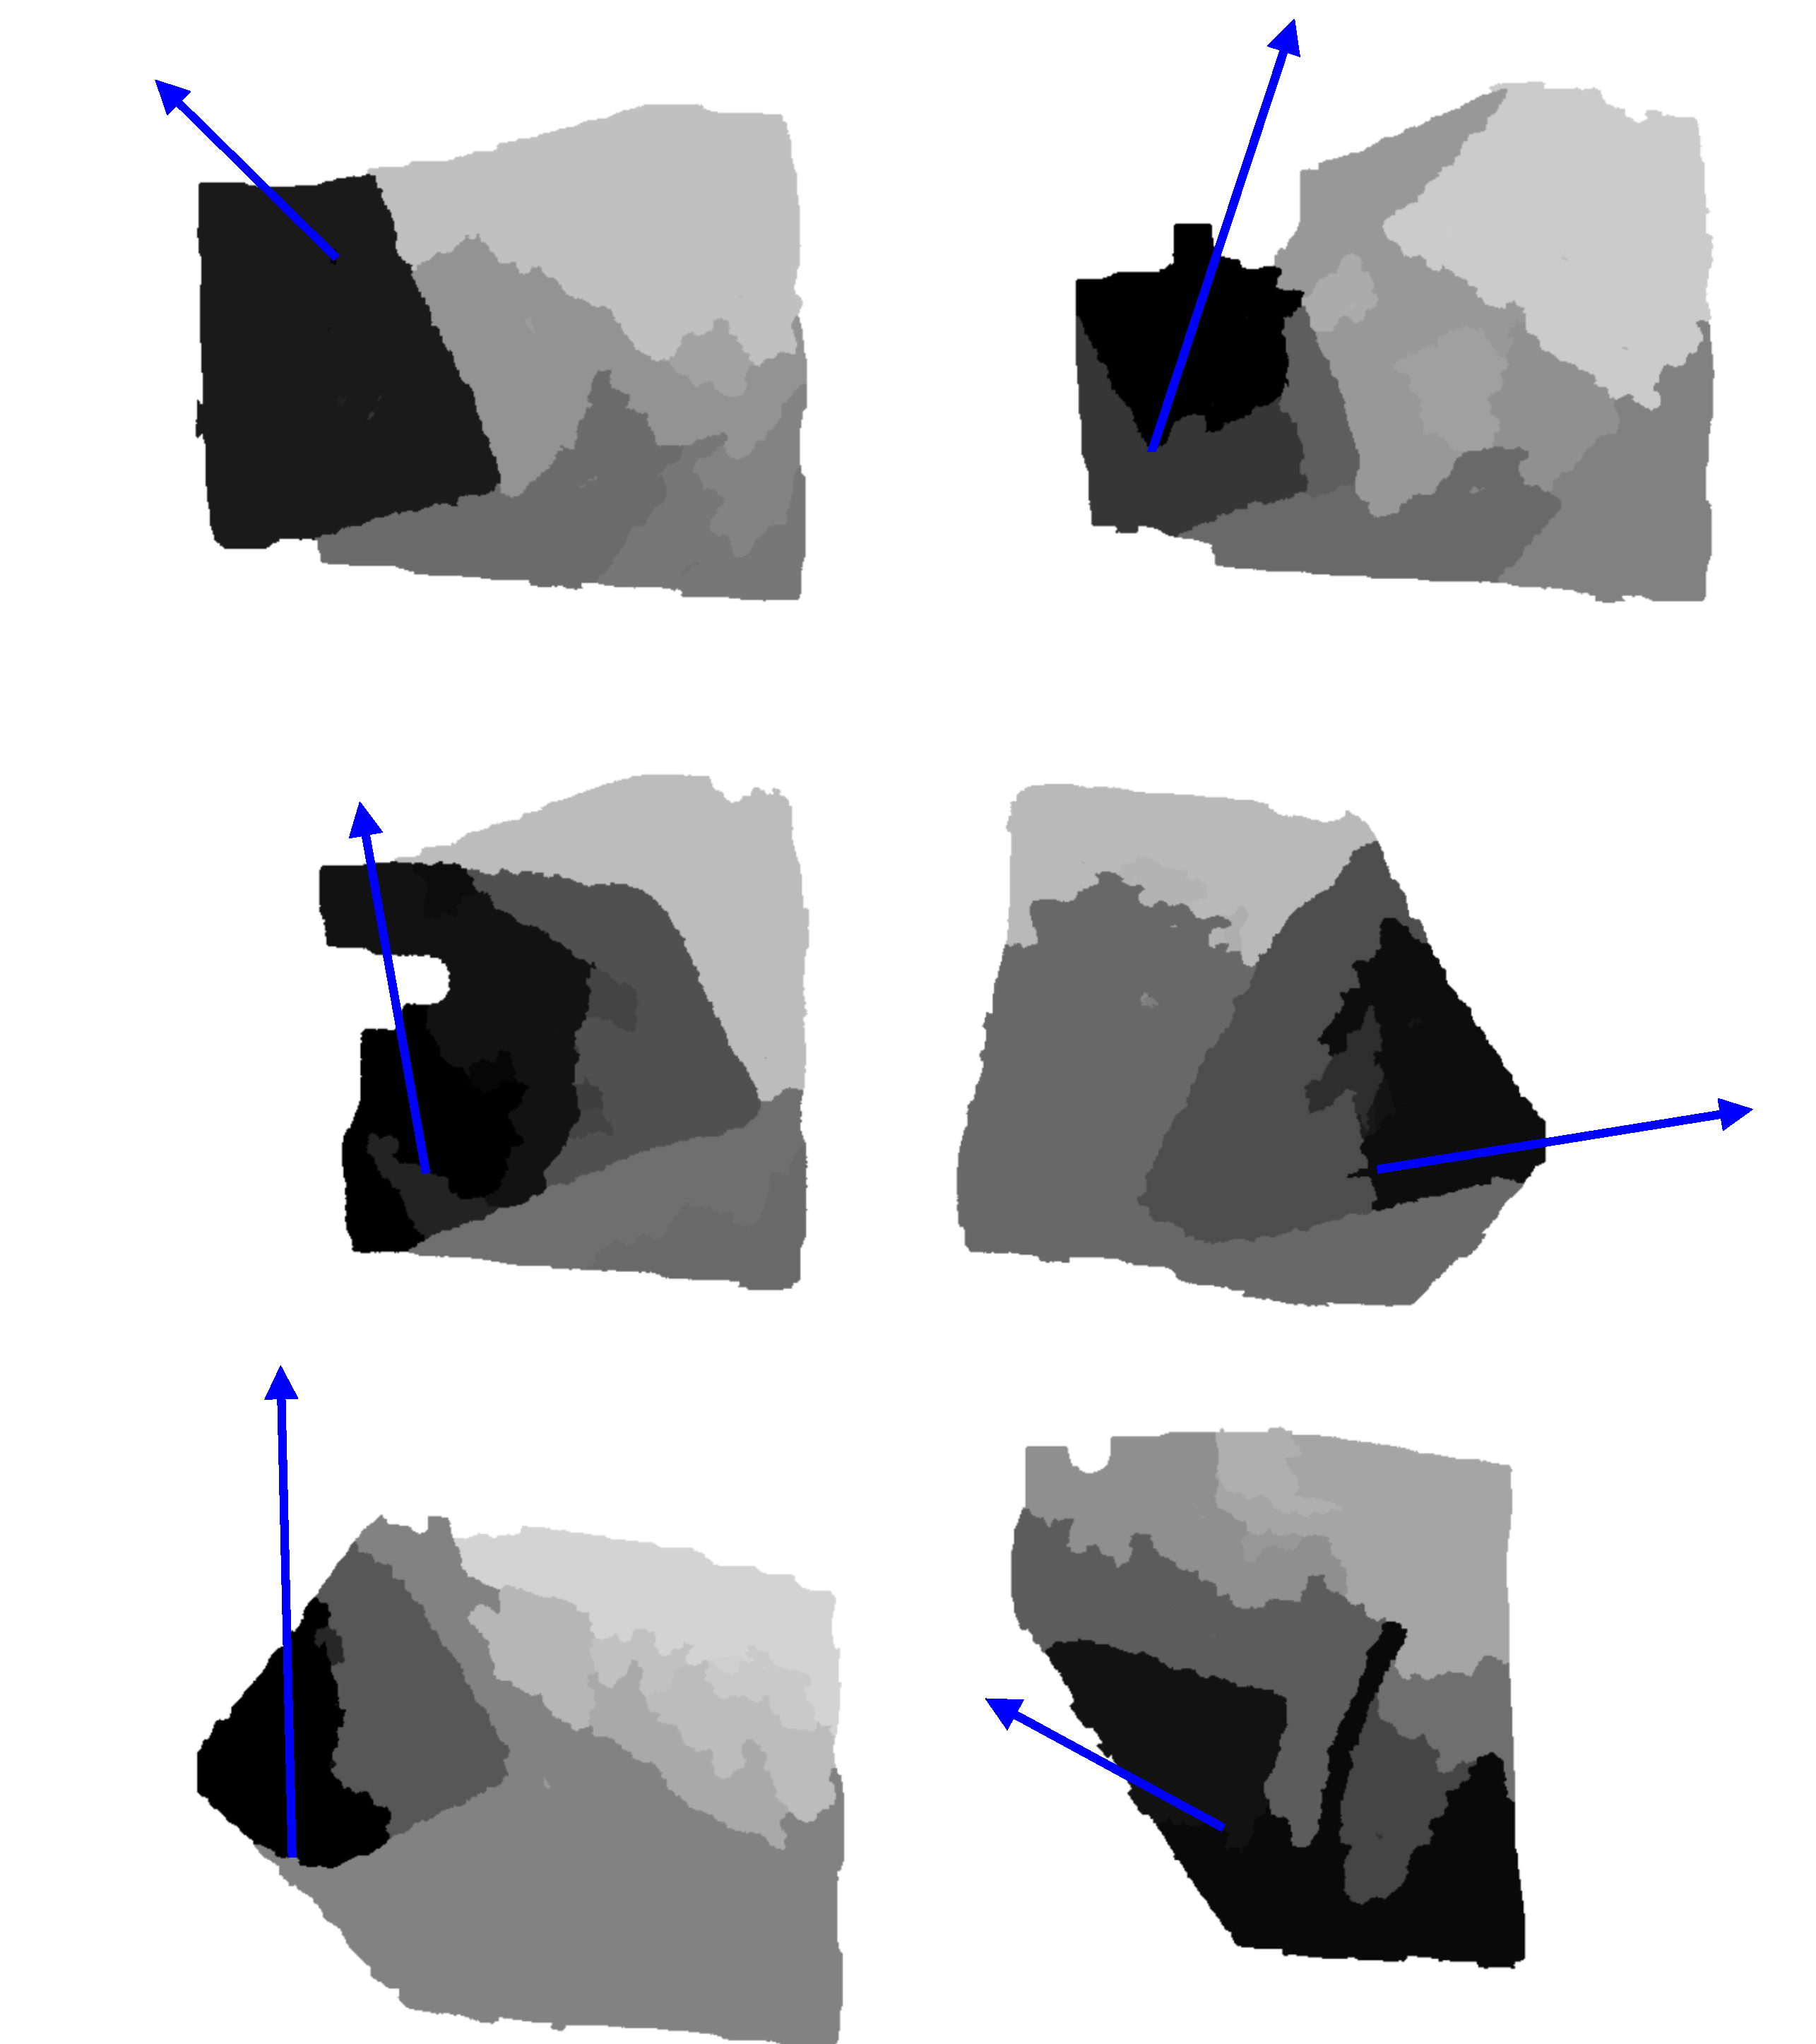
\includegraphics[width=\textwidth]
    {figures/directions.pdf}
    \caption{Final directions calculated for each garment provided to the system. Each arrow departs where the robot should pick the fold and arrives where it should be placed.}
    \label{fig:directions}
\end{figure}



	\chapter{Experiments and results}
\label{experiments_and_results}

The algorithm presented in this work was implemented and evaluated through several experiments using our own garment dataset, as well as validated with experiments using a real robot. This chapter is devoted to explain the experiments performed using the algorithm presented in this thesis. It includes the implementation details, the evaluation dataset and experiments details and the validation experiments description. It also includes the results drawn from the different experiments performed.

\section{Implementation details}
\label{experiments:implementation}
The software implementation for this thesis is divided into three different parts dedicated to data obtention, data processing (the algorithm itself) and results evaluation. 

The first part is in charge of communication with the sensor with the objective of extracting the depth data. This communication is performed using YARP \cite{metta2006yarp}. YARP is a set of libraries, protocols, and tools that leverages many common tasks required for a humanoid robot to work. The tasks include actuator control and command, communications with the robot and between software parts, and accessing to data captured from different common sensors, such as depth sensors.

The second main part is the implementation of the unfolding algorithm. This implementation was executed using Python\footnote{\url{http://www.python.org}} as our language of choice. Python is a programming language that allows a quick development of prototype software, and counts with a large collection of external modules to perform several tasks, from math calculations to computer vision. The implementation is divided into 3 consecutive stages, and within each of the stages, each step is also isolated and executed consecutively, to avoid tight coupling between the different stages and steps of the algorithm. This will allow the authors to quickly explore and test alternative implementations for each of the stages, or even for a single step within any stage, and check whether they improve the performance of the algorithm or they do not cause any significant improvement. Our current implementation is based on two different computer vision libraries: OpenCV\footnote{\url{http://www.opencv.org}} and Scikit-image\footnote{\url{http://scikit-image.org}}. We chose to use both since during the development of this work several algorithms were tested, and each library contains only a subset of those algorithms. In the latest version, OpenCV is used for basic computer vision and Scikit-image for more advanced algorithms such as Watershed \footnote{\url{http://scikit-image.org/docs/dev/auto_examples/plot_watershed.html}} and other superpixel-based clustering methods. The implementation also relies heavily on Numpy\footnote{\url{http://www.numpy.org/}}. Numpy is the \textit{de facto} Python library for scientific computing, and all the operations with trajectories and unfolding paths required in our work, such as line intersections or line perpendicularity, were implemented using the mathematical functions present on Numpy. We are releasing our unfolding algorithm implementation to the public with an Open Source license, and it is already available online\footnote{\url{https://github.com/roboticslab-uc3m/textiles}}.


For the evaluation of the results a Graphical User Interface (GUI) was created using Python and PySide\footnote{\url{https://wiki.qt.io/PySide}} (LGPL Qt bindings for Python). As it is shown in figure \ref{fig:gui}, this GUI is composed of a main view where results are presented and 3 buttons to indicate the 3 possible evaluations that each result can be given (\fail{}, \good{} and \great{}). These evaluations will be explained in further detail later in this chapter, in section \comment{\ref{}.} 

\begin{figure}[thpb]
    \centering
    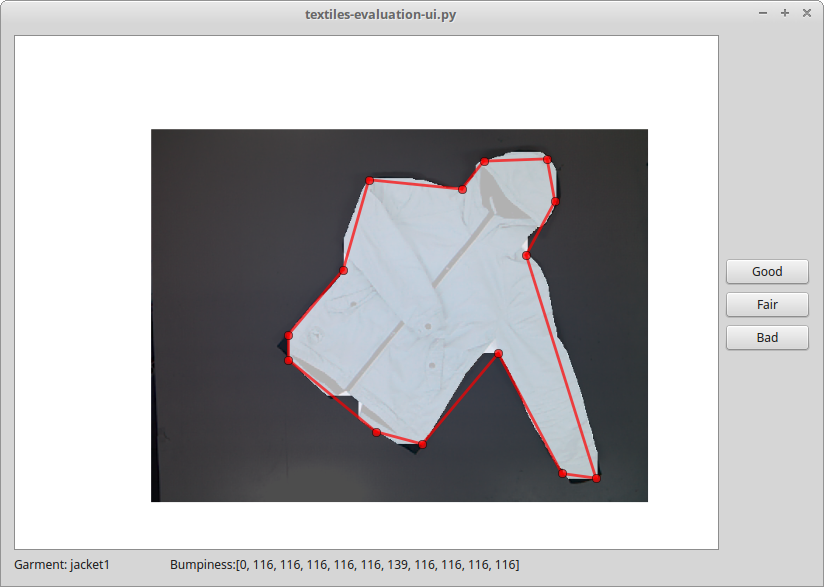
\includegraphics[width=0.7\textwidth]
    {figures/evaluation-gui.png}
    \caption[GUI]
    {GUI}
    \label{fig:gui}
\end{figure}


Some extra information is also provided in the bottom part of the GUI, such as the name of the garment being evaluated and the bumpiness value for all the candidate unfold paths. Results from each of the 3 stages of our algorithm are first calculated by running the algorithm with all the garment samples. Then, these results are presented consecutively for all the samples in the dataset, and if any of them is evaluated as \fail{}, the remaining ones are skipped for that garment, and automatically evaluated as \discarded{}. All these evaluations are logged and when there are no results left to score, the statistic analysis of the logged evaluations is performed and presented to the evaluator. 

\section{Algorithm Evaluation}
\label{experiments:evaluation}

\comment{Bla, bla, bla... evaluation, bla, bla, bla}

\subsection{Garment Dataset}
\label{experiments:dataset}

To test the computer vision algorithm, a garment dataset was crafted\footnote{\url{http://tinyurl.com/garments-birdsEye-zip}}. Other garment datasets already existed, such as the ones provided by the CloPeMa project\footnote{\url{http://clopema.felk.cvut.cz/public_data.html}}, but they were not suitable to test our algorithm, since these datasets are mainly focused on modeling and folding garments once they are already extended. 

Our dataset is composed of 120 samples of different folds in garments from 6 different categories: skirt, jacket, pants, polo, robe and hoodie. Each category set is composed by 20 samples, 10 of which present one fold and 10 of which present two folds in the garment. This data was obtained using an ASUS Xtion PRO LIVE with RGB and depth channels set at 640x480 resolution. The sensor is placed on top of the working surface providing a bird's eye view over the garment folding environment, with its image plane almost parallel to the working surface.

\comment{Lorem ipsum dolor sit amet, consectetur adipiscing elit. Donec a diam lectus. Sed sit amet ipsum mauris. Maecenas congue ligula ac quam viverra nec consectetur ante hendrerit. Donec et mollis dolor. Praesent et diam eget libero egestas mattis sit amet vitae augue. Nam tincidunt congue enim, ut porta lorem lacinia consectetur. Donec ut libero sed arcu vehicula ultricies a non tortor. Lorem ipsum dolor sit amet, consectetur adipiscing elit. Aenean ut gravida lorem. Ut turpis felis, pulvinar a semper sed, adipiscing id dolor. Pellentesque auctor nisi id magna consequat sagittis. Curabitur dapibus enim sit amet elit pharetra tincidunt feugiat nisl imperdiet. Ut convallis libero in urna ultrices accumsan. Donec sed odio eros. Donec viverra mi quis quam pulvinar at malesuada arcu rhoncus. Cum sociis natoque penatibus et magnis dis parturient montes, nascetur ridiculus mus. In rutrum accumsan ultricies. Mauris vitae nisi at sem facilisis semper ac in est.}

\subsection{Experiments}
\label{experiments:experiments}

Fig. \ref{fig:results} shows the final output of the algorithm and the computed unfolding directions for 4 garments of each of the 6 categories.

\begin{figure}[htbp]
	\centering
	%%%%%%%%%%%%%%%%%%%%%%%%%%%%%%%%%% FigA %%%%%%%%%%%%%%%%%%%%%%%%%%%%%%%%%%%%%%%%%%%%%
	\begin{subfigure}[l]{\bigtablewidth}
	    \centering
    	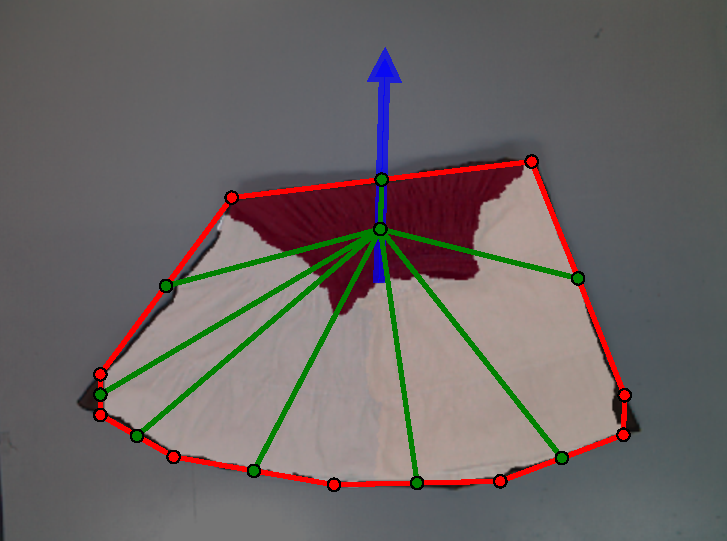
\includegraphics[width=\textwidth]
    	{figures/results/skirt3-pnp.pdf}
	\end{subfigure}
	~
	\begin{subfigure}[r]{\bigtablewidth}
	    \centering
    	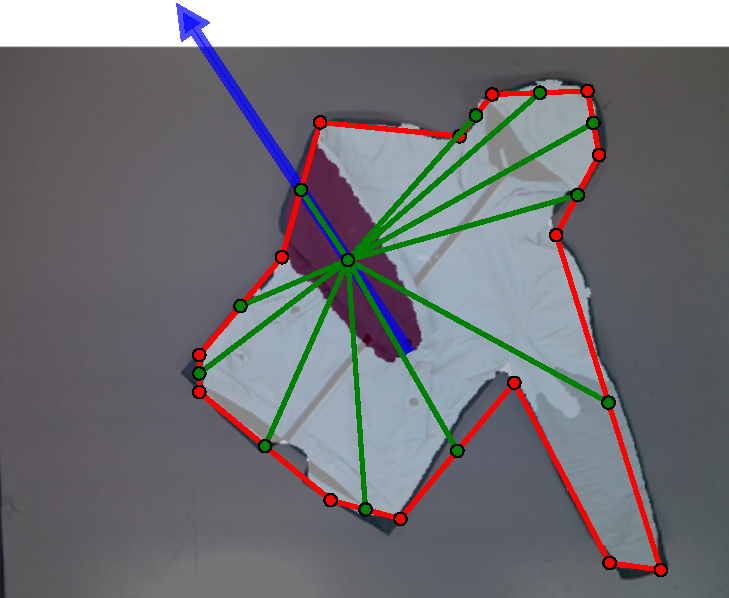
\includegraphics[width=\textwidth]
    	{figures/results/jacket1-pnp.pdf}
	\end{subfigure}
	~
    \begin{subfigure}[l]{\bigtablewidth}
	    \centering
    	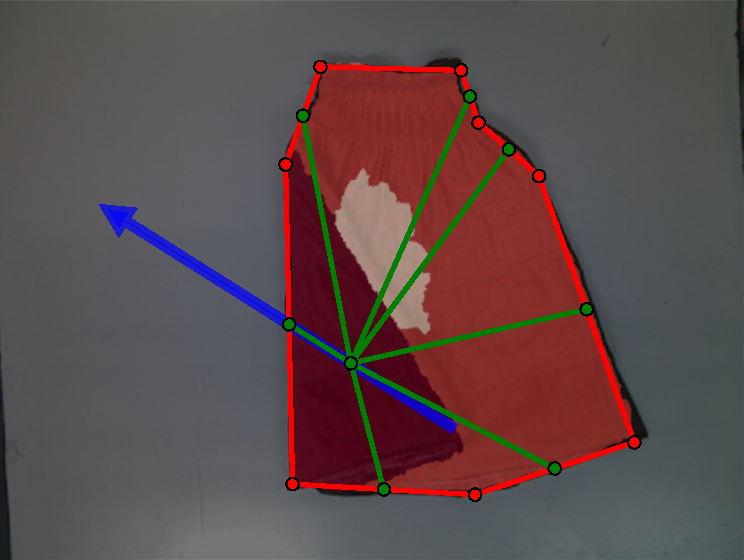
\includegraphics[width=\textwidth]
    	{figures/results/skirt7-pnp.pdf}
	\end{subfigure}
	~
    \begin{subfigure}[r]{\bigtablewidth}
	    \centering
    	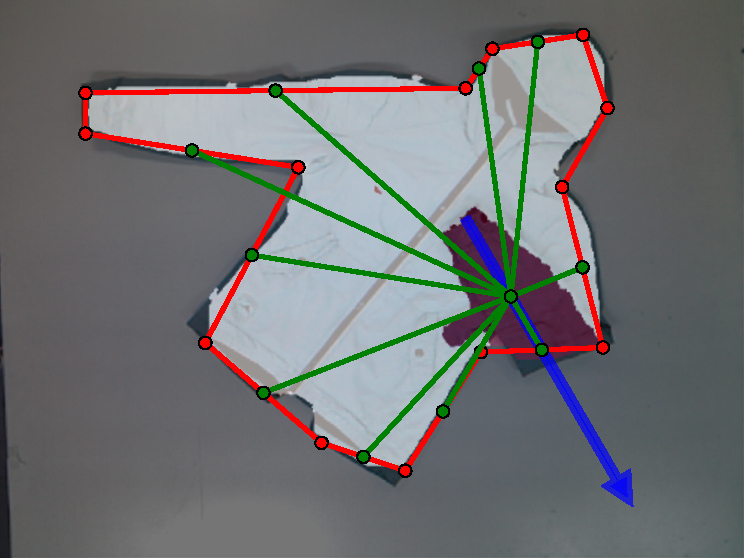
\includegraphics[width=\textwidth]
    	{figures/results/jacket2-pnp.pdf}
	\end{subfigure}
	~
    \begin{subfigure}[l]{\bigtablewidth}
	    \centering
    	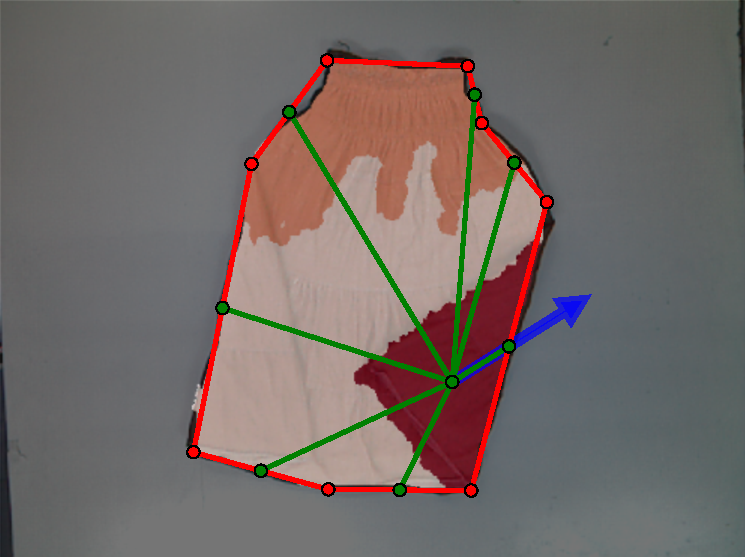
\includegraphics[width=\textwidth]
    	{figures/results/skirt13-pnp.pdf}
	\end{subfigure}
	~
    \begin{subfigure}[r]{\bigtablewidth}
	    \centering
    	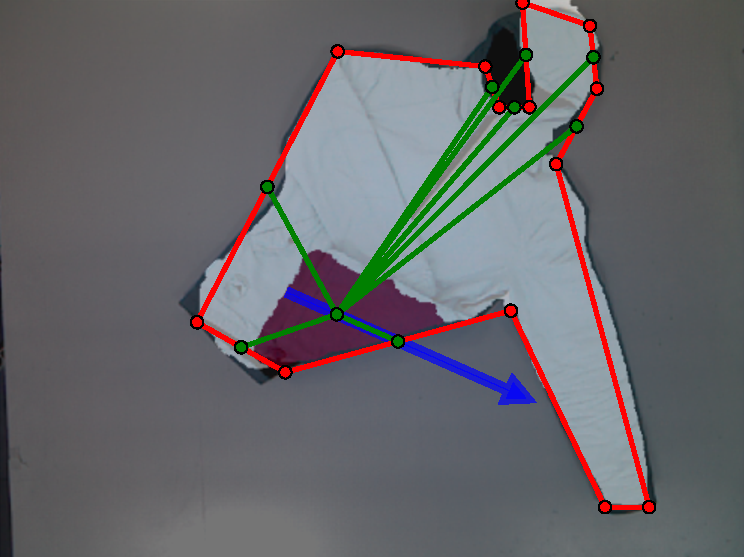
\includegraphics[width=\textwidth]
		{figures/results/jacket12-pnp.pdf}
	\end{subfigure}
	~
    \begin{subfigure}[l]{\bigtablewidth}
	    \centering
    	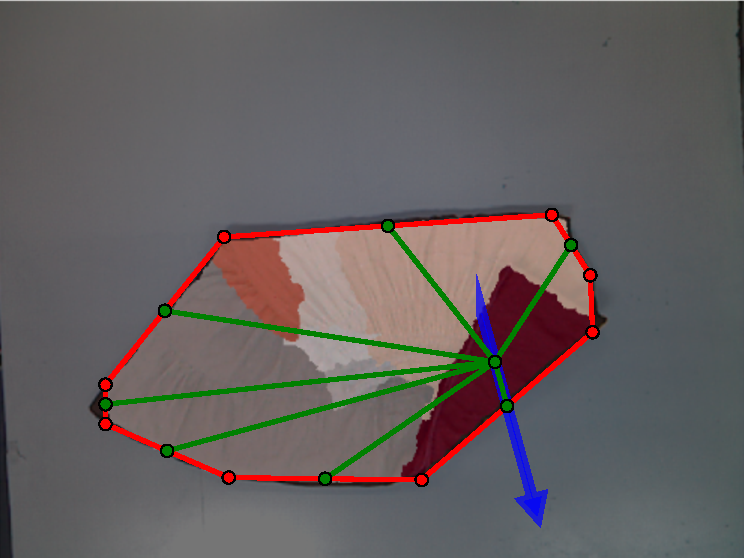
\includegraphics[width=\textwidth]
    	{figures/results/skirt19-pnp.pdf} 
	\end{subfigure}
	~
    \begin{subfigure}[r]{\bigtablewidth}
	    \centering
    	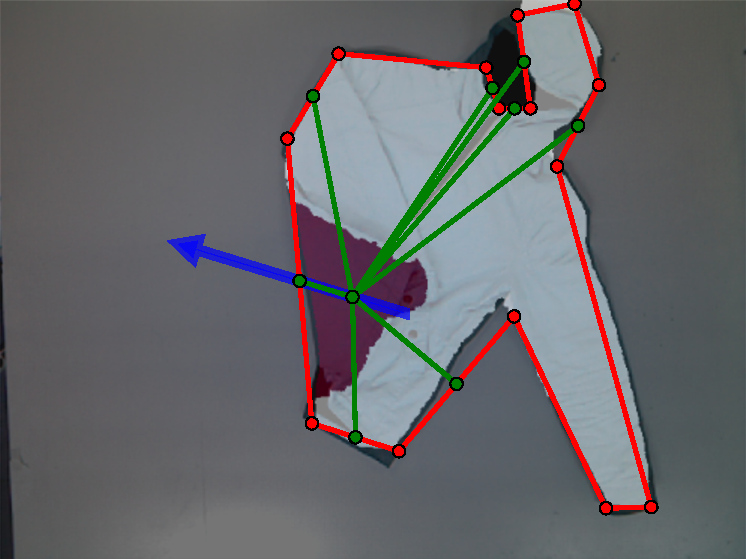
\includegraphics[width=\textwidth]
		{figures/results/jacket13-pnp.pdf}    	
	\end{subfigure}
    \caption[Final output of the algorithm and the computed unfolding directions (Skirt and jacket)]
    {Final output of the algorithm and the computed unfolding directions. Each column includes the output corresponding to 4 of the 20 database samples for each of the 6 garment categories considered. This figure includes the categories Skirt and Jacket.}
    \label{fig:results}
\end{figure}

\begin{figure}[htbp]
	\centering
	%%%%%%%%%%%%%%%%%%%%%%%%%%%%%%%%%% FigB %%%%%%%%%%%%%%%%%%%%%%%%%%%%%%%%%%%%%%%%%%%%%
	\begin{subfigure}[l]{\bigtablewidth}
	    \centering
    	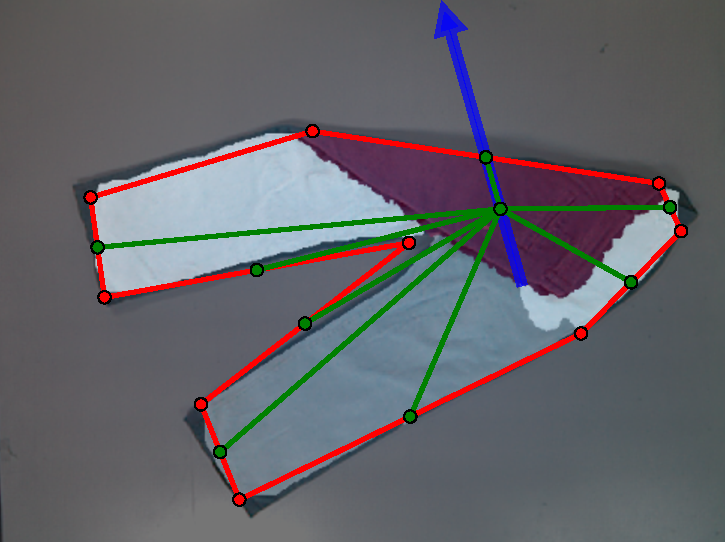
\includegraphics[width=\textwidth]
    	{figures/results/pants7-pnp.pdf}
	\end{subfigure}
	~
	\begin{subfigure}[r]{\bigtablewidth}
	    \centering
    	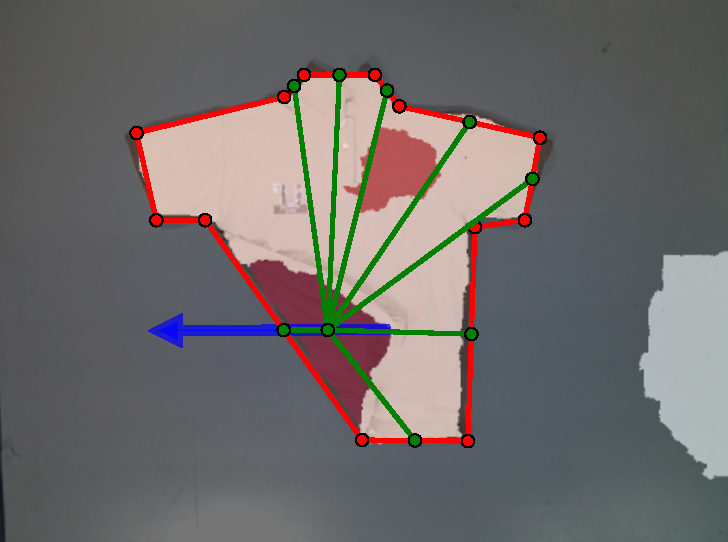
\includegraphics[width=\textwidth]
    	{figures/results/polo1-pnp.pdf}
	\end{subfigure}
	~
    \begin{subfigure}[l]{\bigtablewidth}
	    \centering
    	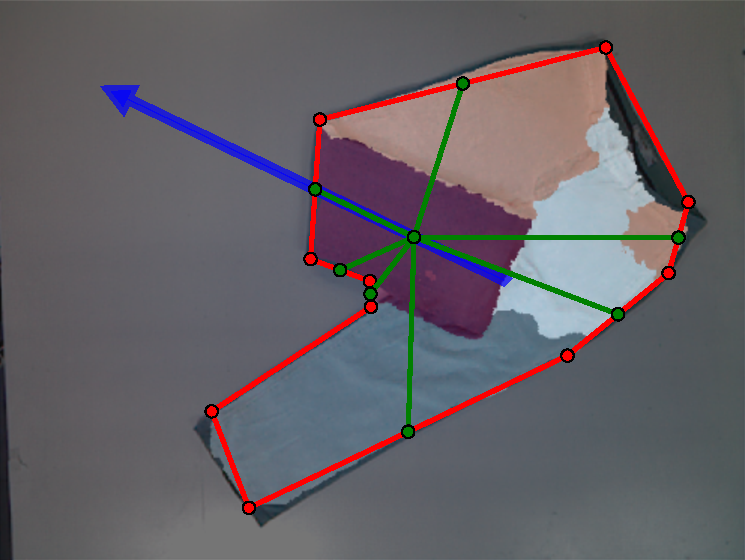
\includegraphics[width=\textwidth]
    	{figures/results/pants8-pnp.pdf}
	\end{subfigure}
	~
    \begin{subfigure}[r]{\bigtablewidth}
	    \centering
    	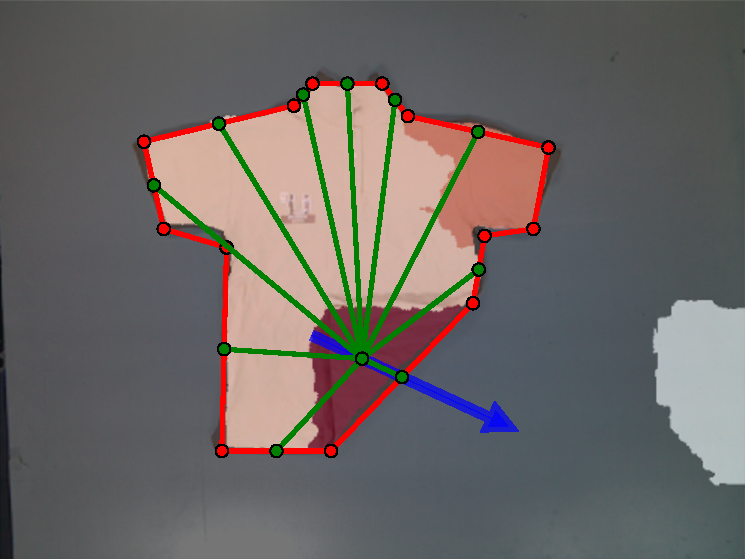
\includegraphics[width=\textwidth]
    	{figures/results/polo2-pnp.pdf}
	\end{subfigure}
	~
    \begin{subfigure}[l]{\bigtablewidth}
	    \centering
    	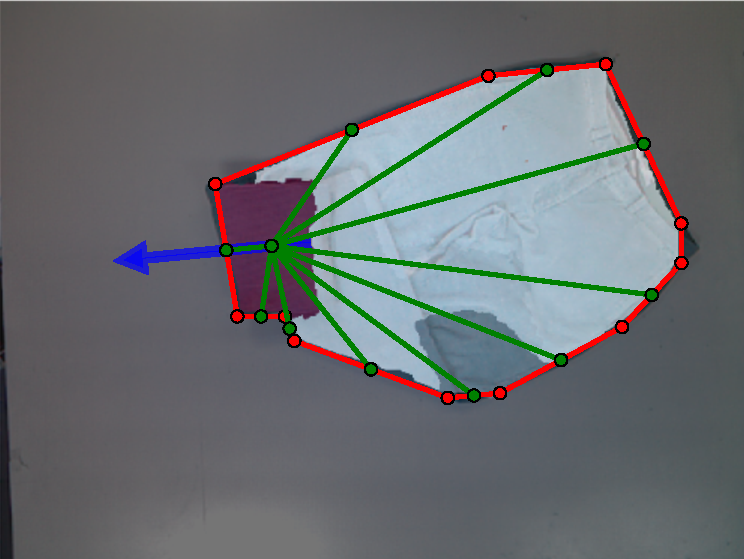
\includegraphics[width=\textwidth]
    	{figures/results/pants14-pnp.pdf}
	\end{subfigure}
	~
    \begin{subfigure}[r]{\bigtablewidth}
	    \centering
    	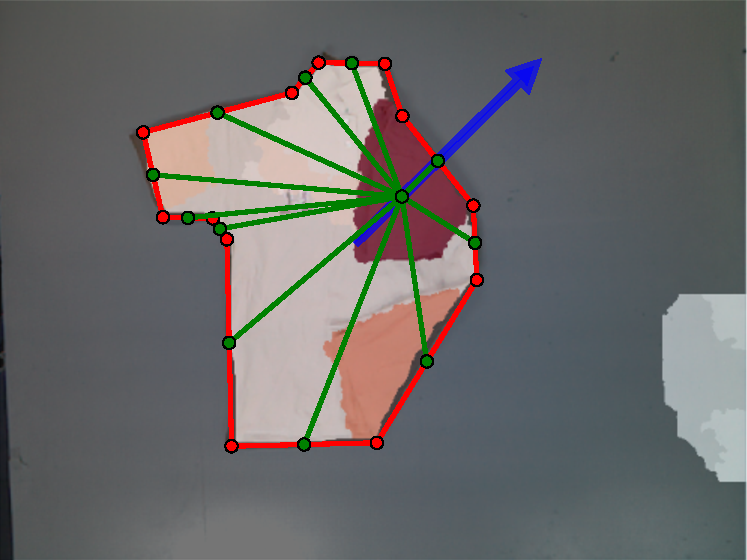
\includegraphics[width=\textwidth]
    	{figures/results/polo13-pnp.pdf}
	\end{subfigure}
	~
    \begin{subfigure}[l]{\bigtablewidth}
	    \centering
    	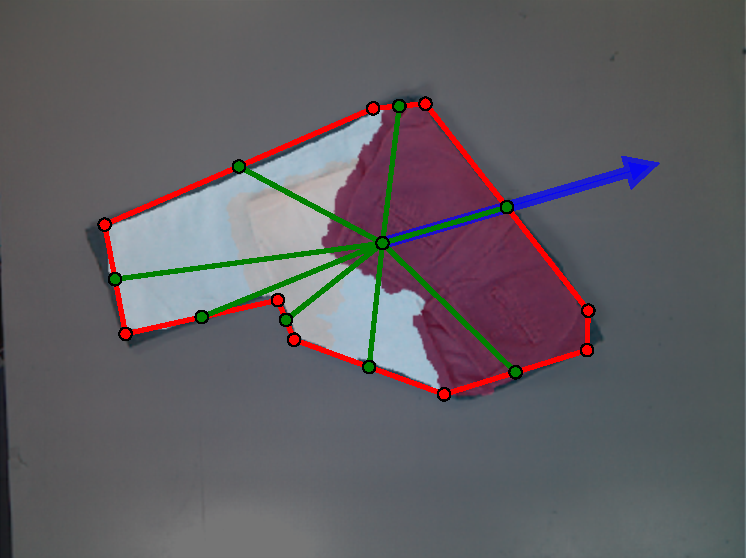
\includegraphics[width=\textwidth]
    	{figures/results/pants15-pnp.pdf}
	\end{subfigure}
	~
    \begin{subfigure}[r]{\bigtablewidth}
	    \centering
    	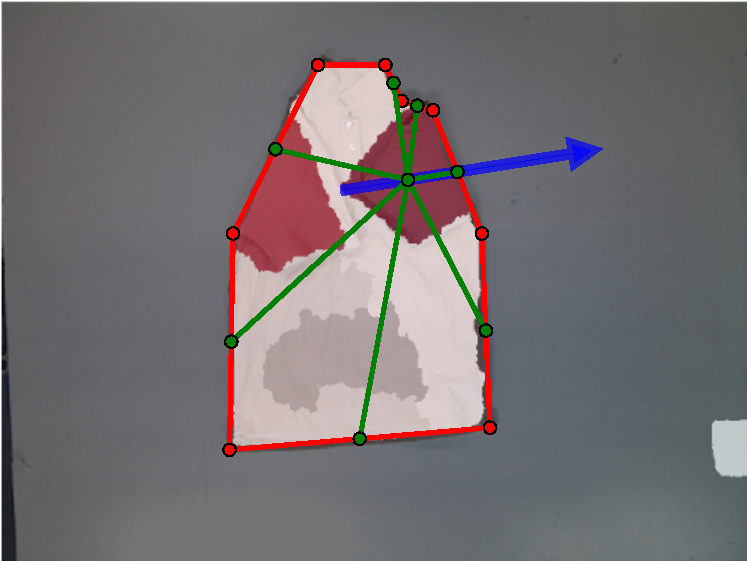
\includegraphics[width=\textwidth]
    	{figures/results/polo15-pnp.pdf}
	\end{subfigure}
	\caption[Final output of the algorithm and the computed unfolding directions (Pants and Polo).]
    {Final output of the algorithm and the computed unfolding directions. Each column includes the output corresponding to 4 of the 20 database samples for each of the 6 garment categories considered.This figure includes the categories Pants and Polo.}
    \label{fig:results2}
\end{figure}

\begin{figure}[htbp]
	\centering
	%%%%%%%%%%%%%%%%%%%%%%%%%%%%%%%%%% FigC %%%%%%%%%%%%%%%%%%%%%%%%%%%%%%%%%%%%%%%%%%%%%
	\begin{subfigure}[l]{\bigtablewidth}
	    \centering
    	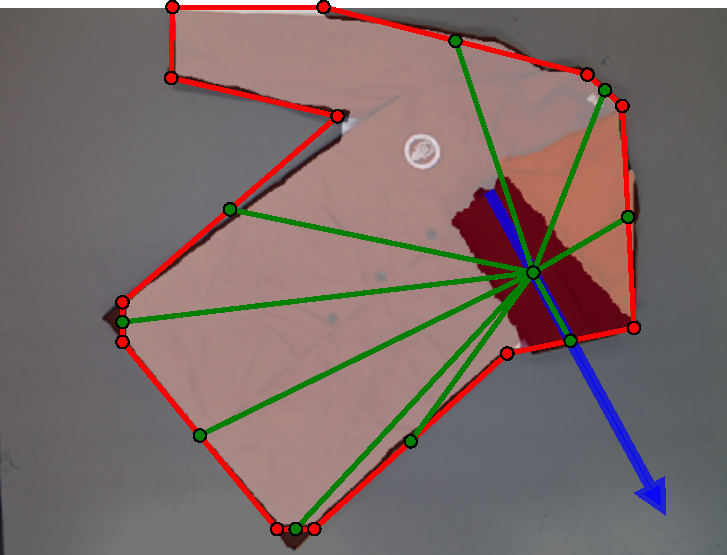
\includegraphics[width=\textwidth]
    	{figures/results/robe4-pnp.pdf}
	\end{subfigure}
	~
    \begin{subfigure}[r]{\bigtablewidth}
	    \centering
    	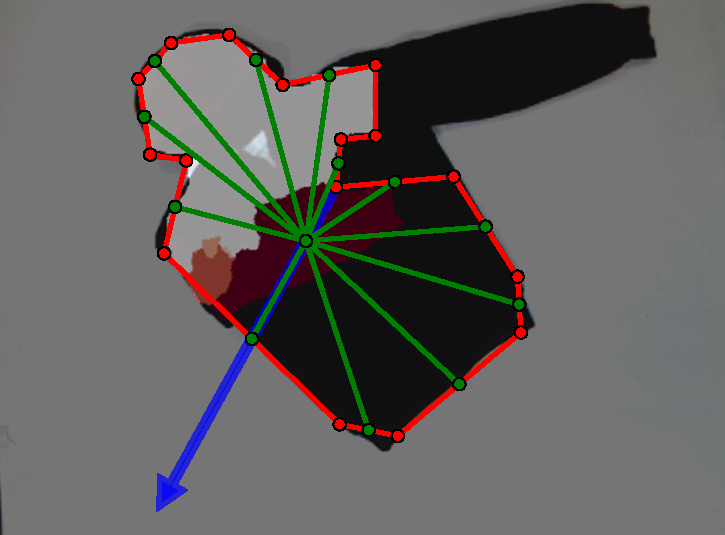
\includegraphics[width=\textwidth]
    	{figures/results/hoodie1-pnp.pdf}
	\end{subfigure}
	~
    \begin{subfigure}[l]{\bigtablewidth}
	    \centering
    	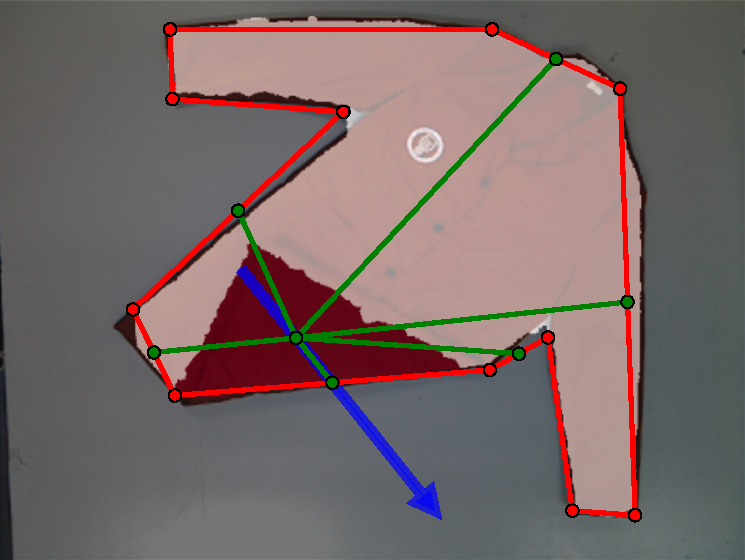
\includegraphics[width=\textwidth]
    	{figures/results/robe8-pnp.pdf}
	\end{subfigure}
	~
    \begin{subfigure}[r]{\bigtablewidth}
	    \centering
    	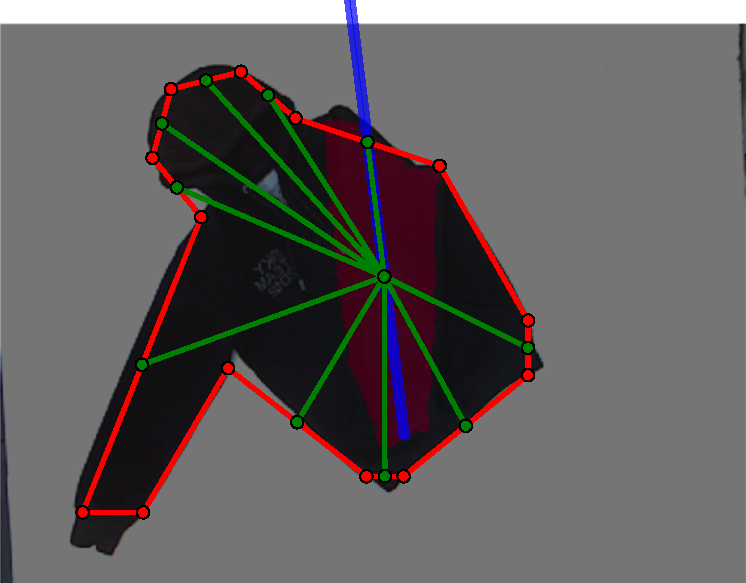
\includegraphics[width=\textwidth]
    	{figures/results/hoodie9-pnp.pdf}
	\end{subfigure} 
	~
	\begin{subfigure}[l]{\bigtablewidth}
	    \centering
    	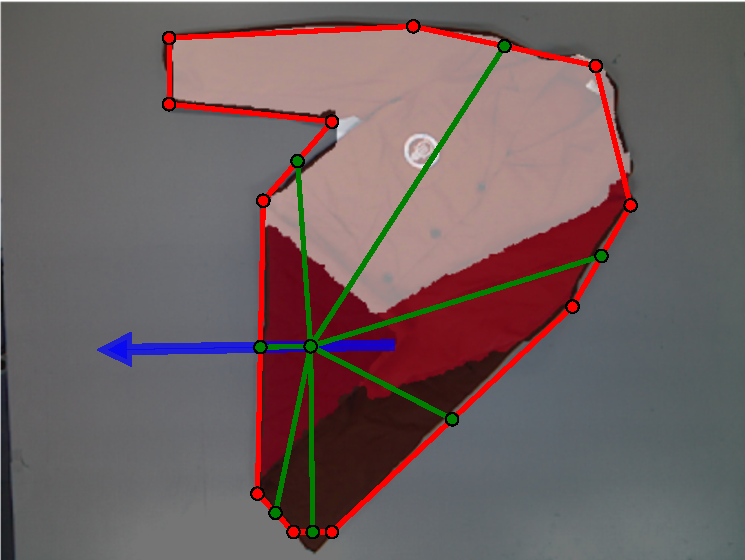
\includegraphics[width=\textwidth]
    	{figures/results/robe15-pnp.pdf}
	\end{subfigure}
	~
    \begin{subfigure}[r]{\bigtablewidth}
	    \centering
    	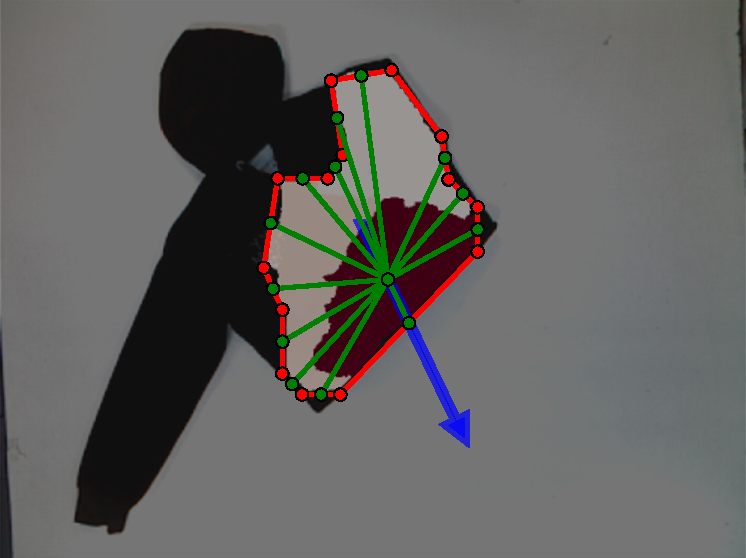
\includegraphics[width=\textwidth]
    	{figures/results/hoodie14-pnp.pdf}    	
	\end{subfigure}
	~
    \begin{subfigure}[l]{\bigtablewidth}
	    \centering
    	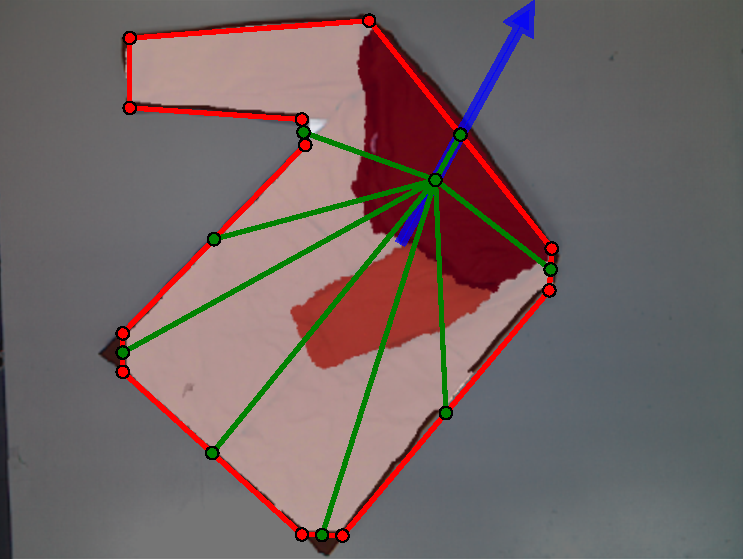
\includegraphics[width=\textwidth]
    	{figures/results/robe19-pnp.pdf}
	\end{subfigure}
	~
    \begin{subfigure}[r]{\bigtablewidth}
	    \centering
    	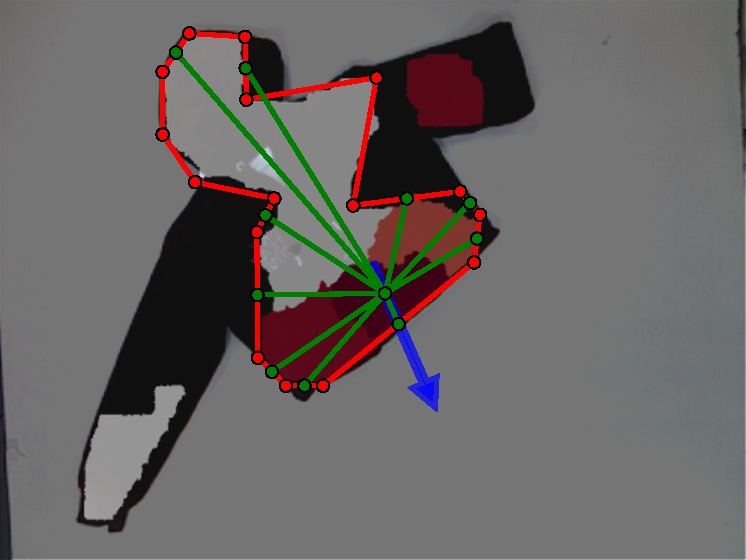
\includegraphics[width=\textwidth]
    	{figures/results/hoodie16-pnp.pdf}
	\end{subfigure} 
    \caption[Final output of the algorithm and the computed unfolding directions (Robe and Hoodie).]
    {Final output of the algorithm and the computed unfolding directions. Each column includes the output corresponding to 4 of the 20 database samples for each of the 6 garment categories considered. This figure includes the categories Robe and Hoodie.}
    \label{fig:results3}
\end{figure}

For evaluating the algorithm, a scoring metric has been established. The criteria for the scoring is qualitative, due to the lack of an objective ground truth to provide quantitative comparisons. The output of each stage is manually classified into one of the following categories: \fail{}, \good{}, \great{} and \discarded{}. Results from one stage that prevent the next one to work properly are classified as \fail{}, and the next stages for that item are classified as \discarded{} and skipped. Results that are not perfect, but allow the next stage to compute its output are classified as \good{}. Note that the \good{} score in the last stage means that the robot could unfold it, but it is not the optimal path. Finally, perfect results for a stage are given the \great{} score. Table \ref{table:table} shows the raw data of this scoring, indicating the amount of samples that received each score at a given stage for each category.


\begin{table}[htbp]
\centering
\begin{tabular}{|c||c|c c c c|}
\hline 
 & Stage & \fail & \good & \great & \discarded \\ 
\hline \hline
 & Segmentation & 0 & 0 & 20 & 0 \\ 
Skirt & Clustering & 3 & 6 & 11 & 0 \\ 
 & Pick \& Place & 5 & 5 & 7 & 3 \\ 
\hline \hline
 & Segmentation & 0 & 9 & 11 & 0 \\ 
Jacket & Clustering & 8 & 8 & 4 & 0 \\ 
 & Pick \& Place & 3 & 3 & 6 & 8 \\ 
\hline \hline
 & Segmentation & 1 & 1 & 18 & 0 \\ 
Pants & Clustering & 7 & 5 & 7 & 1 \\ 
 & Pick \& Place & 8 & 1 & 3 & 8 \\ 
\hline \hline
 & Segmentation & 0 & 17 & 3 & 0 \\ 
Polo & Clustering & 3 & 13 & 4 & 0 \\ 
 & Pick \& Place & 1 & 4 & 12 & 3 \\ 
\hline \hline
 & Segmentation & 0 & 0 & 20 & 0 \\ 
Robe & Clustering & 5 & 7 & 8 & 0 \\ 
 & Pick \& Place & 3 & 3 & 8 & 6 \\ 
\hline \hline
 & Segmentation & 11 & 3 & 6 & 0 \\ 
Hoodie & Clustering & 6 & 2 & 1 & 11 \\ 
 & Pick \& Place & 3 & 0 & 0 & 17 \\ 
\hline 
\end{tabular} 
\caption{Raw data results of the established scoring metric for each garment category and algorithm stage}
\label{table:table}
\end{table}

A stage by stage analysis is provided in Table \ref{table:table2}. Each cell represents the percent of \good{} and \great{} qualified samples with respect to the amount of samples that actually reached the given stage:

\begin{equation}
cell = \frac{\good + \great}{\fail + \good + \great} \cdot 100 \%
\end{equation}

The Overall performance included in the last row shows the percent of \good{} and \great{} samples taking into account all the samples, including the ones scored as \discarded{}, and corresponds to the product of the percentages of each individual stage, since they are independent events.

\begin{table}[htbp]
\centering
\begin{tabular}{|r||r|r|r|r|r|r||r|}
\hline
	Stage \slash{} Category & Skirt & Jacket & Pants & Polo & Robe & Hoodie & All \\
\hline\hline
   Segmentation         & 100   & 100 &  95   & 100   & 100   & 45   & \textbf{90}\\
   Clustering           &  85   &  60 &  63.2 &  85   &  75   & 33.3 & \textbf{70.4}\\
   Pick \& Place Points &  70.6 &  75 &  33.3 &  94.1 &  78.6 &  0   & \textbf{69.3}\\
   \hline\hline
   Overall              &  60   &  45 &  20   &  80   &    55 &  0   & \textbf{43.3} \\ 
\hline
\end{tabular}
\caption{Results analysis per stage and garment category, expressed in percentage (\%)}
\label{table:table2}
\end{table}

For instance, the Segmentation stage was evaluated as having performed correctly (which includes \good{} and \great{} samples) for 100\% of the Skirt category. With the remaining samples, the Clustering stage performance was evaluated. In this case, within the Skirt category, all of the Skirt samples were evaluated, because they had all passed the previous stage. In this evaluation, 85\% achieved a passing score (\good{} and \great{}). This set of samples was passed on to the Pick \& Place points stage, and for these samples, 70.6\% achieved a passing score within the Skirt category. The Overall algorithm performance for the category is computed as the product of the percentages of three stages: $1 \cdot 0.85 \cdot 0.70 = 60\%$ based on the 20 skirt samples. Table \ref{table:table2} includes an additional column which applies this process based on the evaluation of All the 120 samples of the dataset.

A final set of laboratory experiments to validate the unfolding algorithm have been performed using the full-size humanoid robot TEO \cite{martinez2012teo}. The robot's gripper, designed with passive compliance and relatively large objects in mind (e.g. fruit, bottles, etc), was substituted by a gripper for garment manipulation actuated with hobby servomotors. The garment data was obtained using the ASUS RGB-D sensor in the same configuration (at the ceiling) as for the dataset generation. 

Once the unfolding pick and place points are computed, depth sensor coordinates are converted to the robot root frame. A standard pick and place operation is performed with the final obtained points.


\comment{Lorem ipsum dolor sit amet, consectetur adipiscing elit. Donec a diam lectus. Sed sit amet ipsum mauris. Maecenas congue ligula ac quam viverra nec consectetur ante hendrerit. Donec et mollis dolor. Praesent et diam eget libero egestas mattis sit amet vitae augue. Nam tincidunt congue enim, ut porta lorem lacinia consectetur. Donec ut libero sed arcu vehicula ultricies a non tortor. Lorem ipsum dolor sit amet, consectetur adipiscing elit. Aenean ut gravida lorem. Ut turpis felis, pulvinar a semper sed, adipiscing id dolor. Pellentesque auctor nisi id magna consequat sagittis. Curabitur dapibus enim sit amet elit pharetra tincidunt feugiat nisl imperdiet. Ut convallis libero in urna ultrices accumsan. Donec sed odio eros. Donec viverra mi quis quam pulvinar at malesuada arcu rhoncus. Cum sociis natoque penatibus et magnis dis parturient montes, nascetur ridiculus mus. In rutrum accumsan ultricies. Mauris vitae nisi at sem facilisis semper ac in est.}

\section{Algorithm Validation}
\label{experiments:validation}

\comment{Bla, bla, bla.. validation.. bla, bla, bla} \comment{Lorem ipsum dolor sit amet, consectetur adipiscing elit. Donec a diam lectus. Sed sit amet ipsum mauris. Maecenas congue ligula ac quam viverra nec consectetur ante hendrerit. Donec et mollis dolor. Praesent et diam eget libero egestas mattis sit amet vitae augue. Nam tincidunt congue enim, ut porta lorem lacinia consectetur. Donec ut libero sed arcu vehicula ultricies a non tortor. Lorem ipsum dolor sit amet, consectetur adipiscing elit. Aenean ut gravida lorem. Ut turpis felis, pulvinar a semper sed, adipiscing id dolor. Pellentesque auctor nisi id magna consequat sagittis. Curabitur dapibus enim sit amet elit pharetra tincidunt feugiat nisl imperdiet. Ut convallis libero in urna ultrices accumsan. Donec sed odio eros. Donec viverra mi quis quam pulvinar at malesuada arcu rhoncus. Cum sociis natoque penatibus et magnis dis parturient montes, nascetur ridiculus mus. In rutrum accumsan ultricies. Mauris vitae nisi at sem facilisis semper ac in est.}

\subsection{Experimental Setup}
\label{experiments:expermimental_setup}

The experimental setup consisted of several elements in a laboratory environment: a table, a depth sensor and a humanoid robot. The garment was placed on a white, flat surface, parallel to the floor. Over the garment, an ASUS Xtion PRO LIVE depth sensor was attached to a structure to capture data from a top view. The unfolding operation was performed by our full-body humanoid robot TEO \cite{martinez2012teo}. Figure \ref{fig:experimental_setup} depicts this setup.

\begin{figure}[htbp]
    \centering
    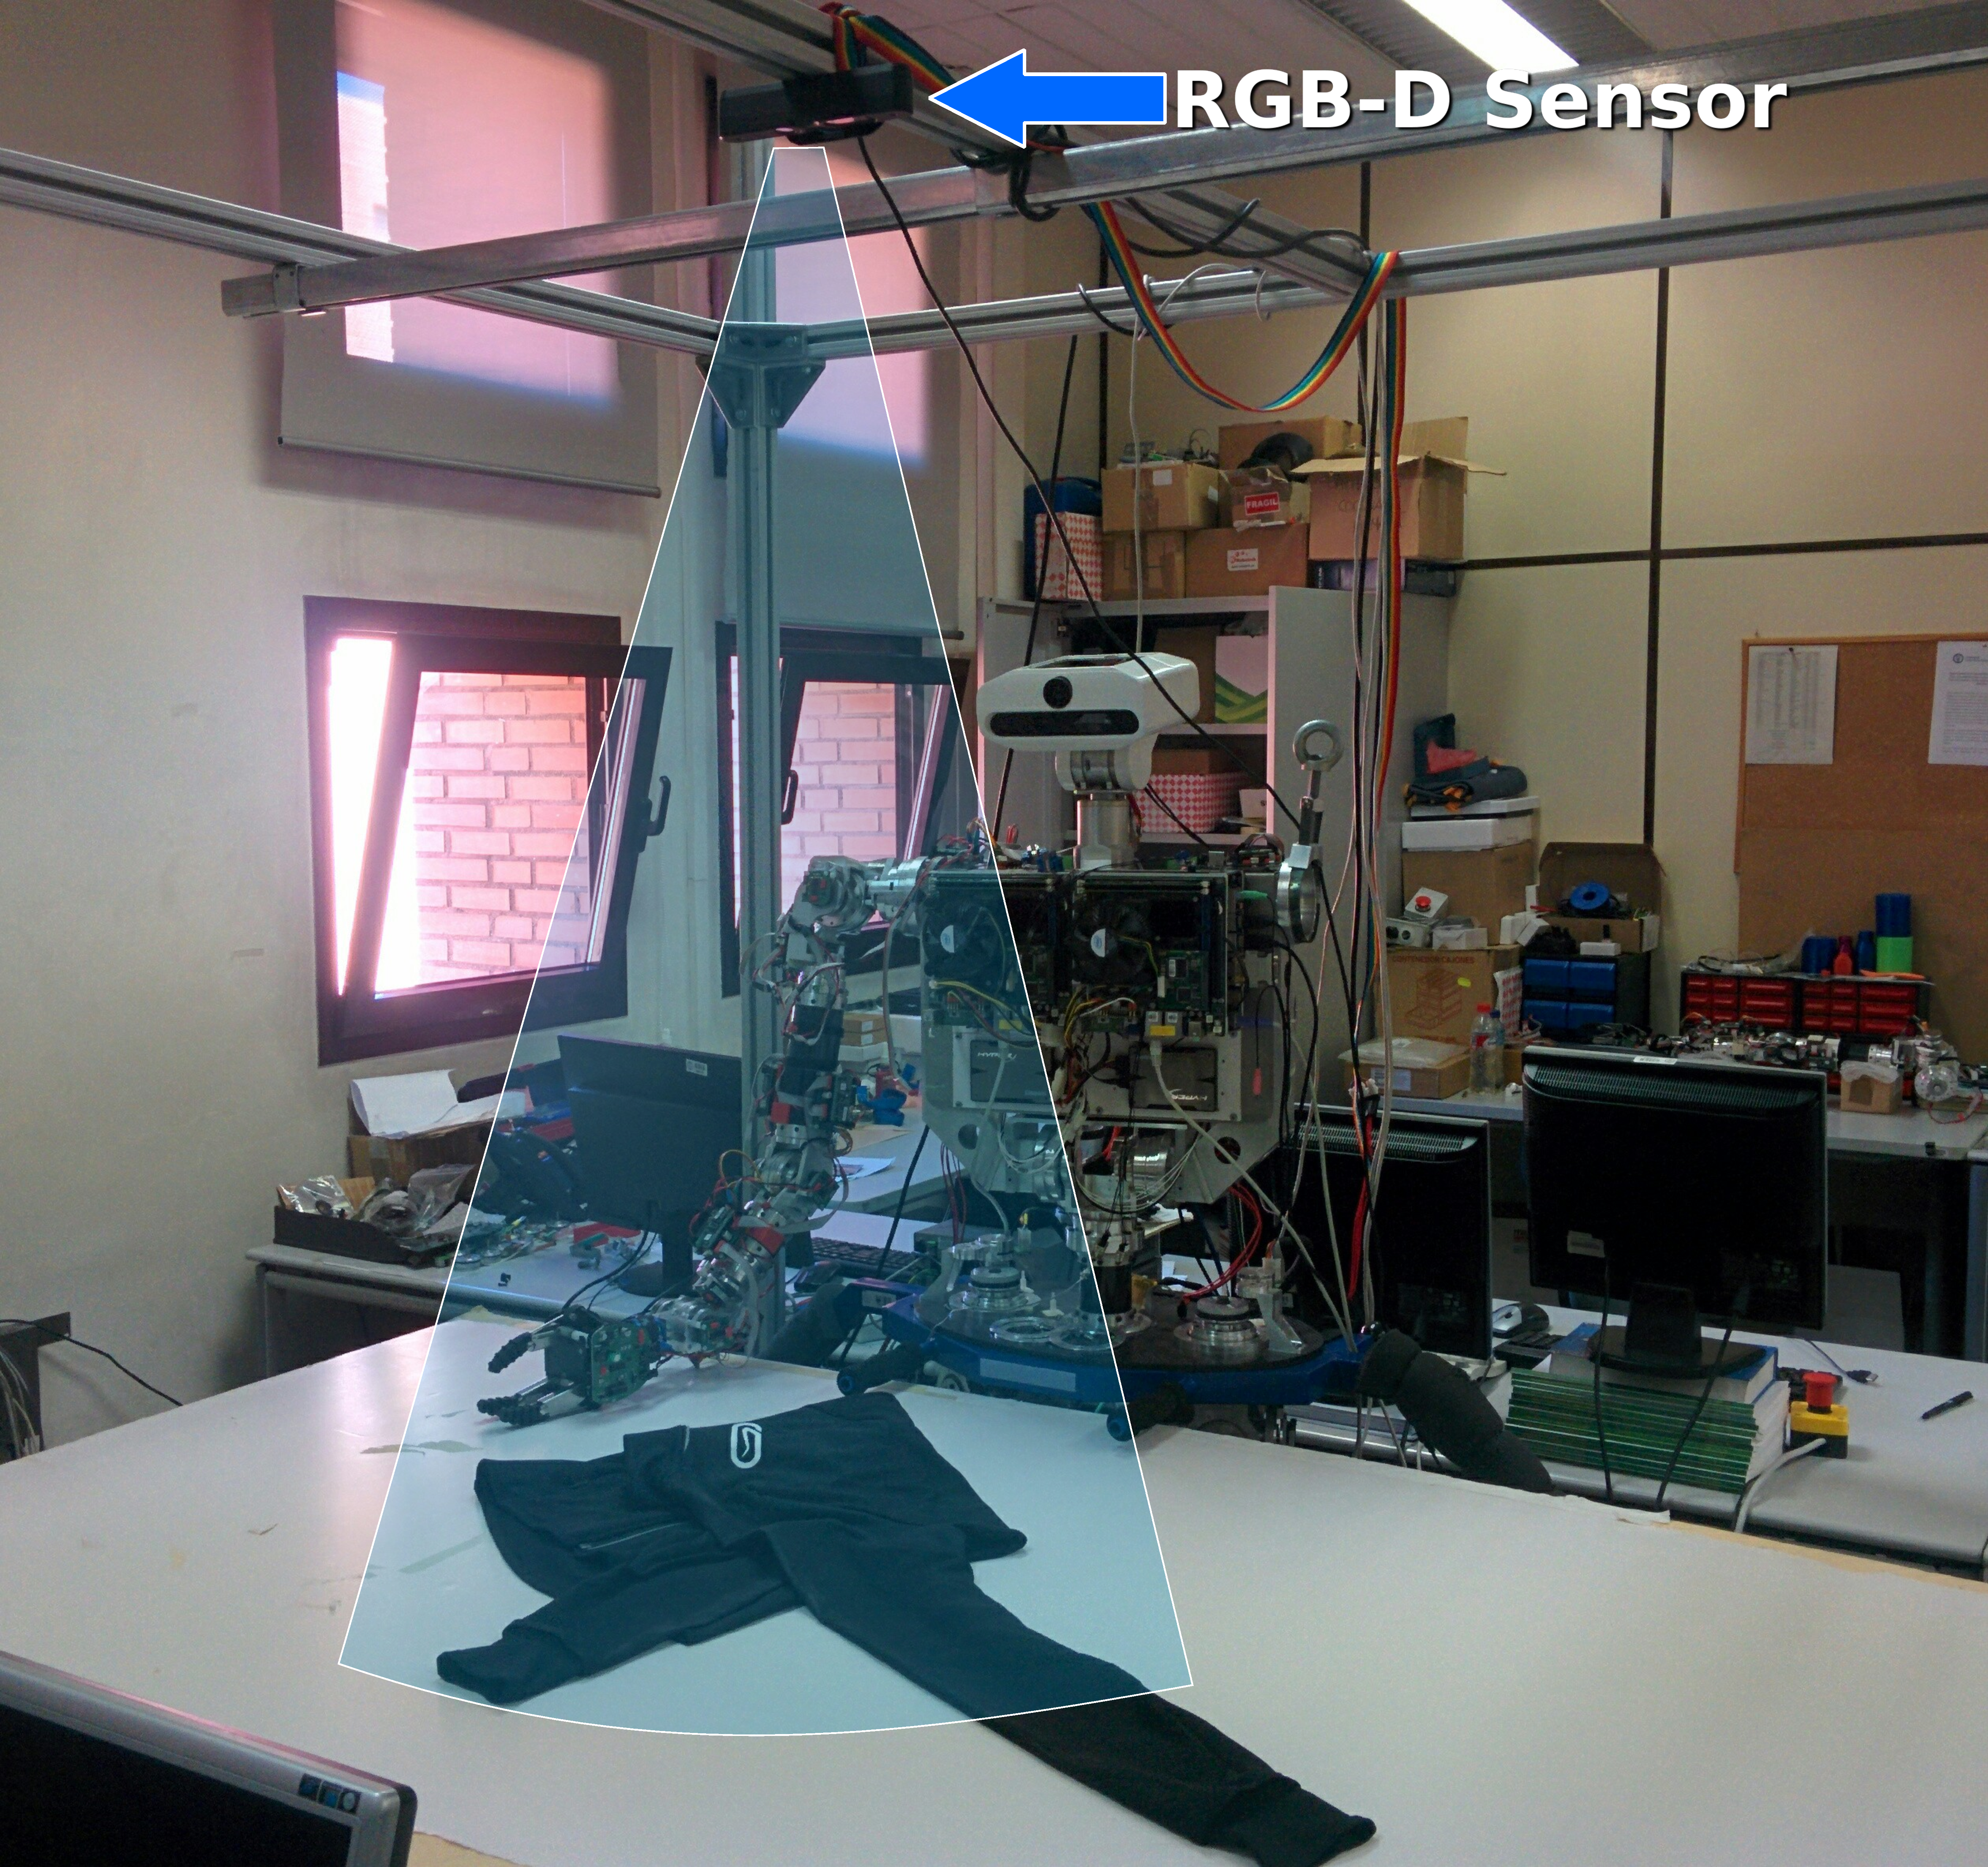
\includegraphics[width=0.8
    \textwidth]{figures/Experimental_setup.pdf}
    \caption[Experimental setup used to test the algorithm]
    {This figure shows the experimental setup used to test the algorithm. The garment rests over a flat white table, with the RGB-D sensor on top. Besides the table, the humanoid robot TEO waits for manipulation trajectories that indicate it how to perform the unfold action.}
    \label{fig:experimental_setup}
\end{figure}

The starting point for testing our algorithm is the data adquisition process. Data is obtained as a point cloud from a ASUS Xtion Pro Live sensor. Then, it is converted to a depth map image for its later analysis. 

This conversion is done by simply using the z component of each point as the depth value for each pixel of the depth image. If there were a known deviation from the surface (affecting perpendicularity), the depth image could be recovered from the point cloud using the instrinsic and extrinsic parameters of the sensor instead. As the sensor is placed on top of the garment, perpendicular to the surface on which the clothing article rests, both methods yield very similar results, as shown in figure \ref{fig:point_cloud_and_depth_image}.

\begin{figure}[htbp]
	\centering
    \begin{subfigure}[l]{0.49\textwidth}
	    \centering
    	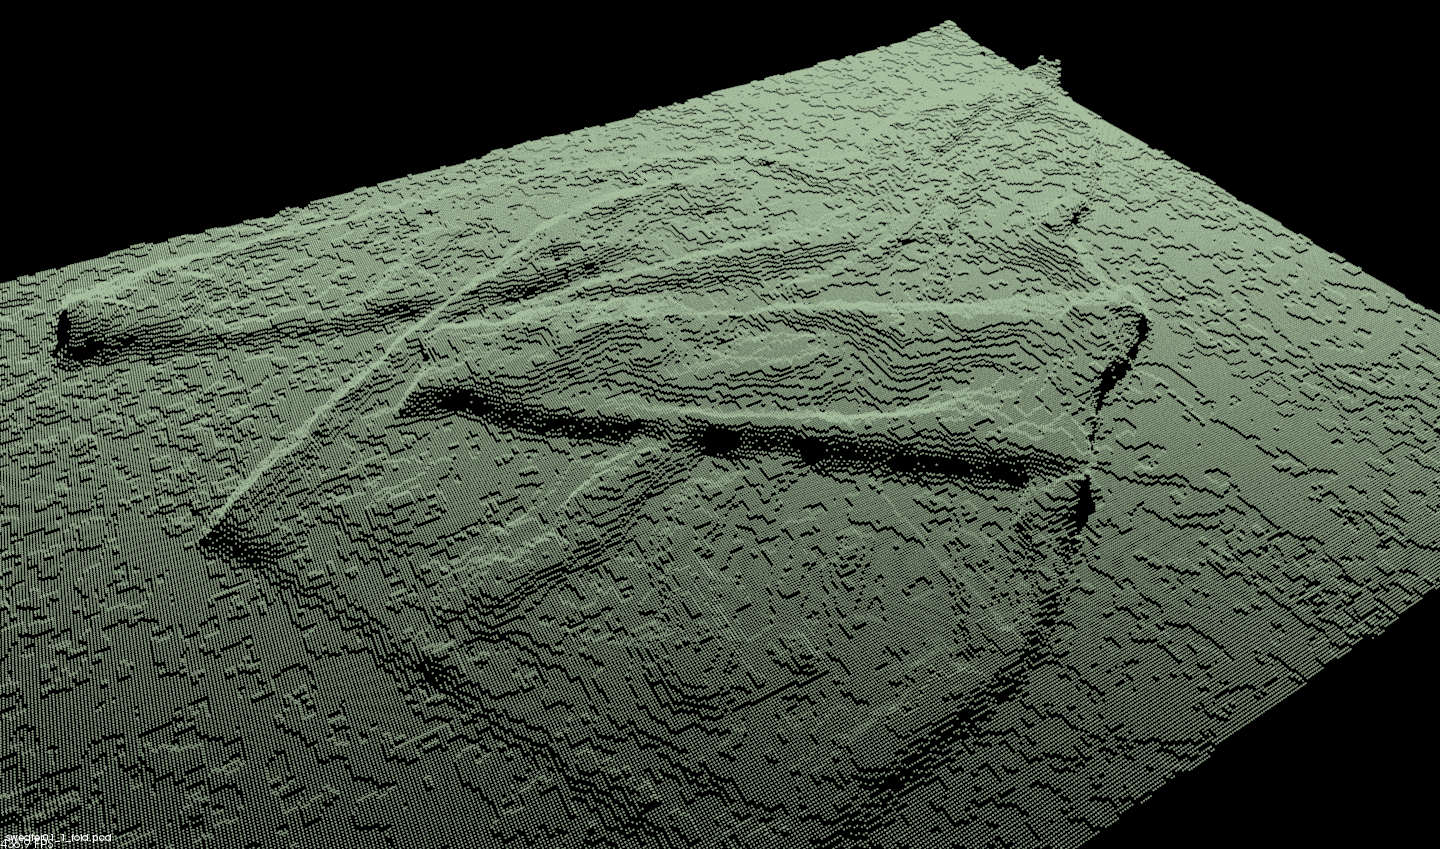
\includegraphics[width=\textwidth]
    	{figures/point-cloud-01.png}
    	\caption{3D Point cloud}
	\end{subfigure}
	~
    \begin{subfigure}[r]{0.49\textwidth}
	    \centering
    	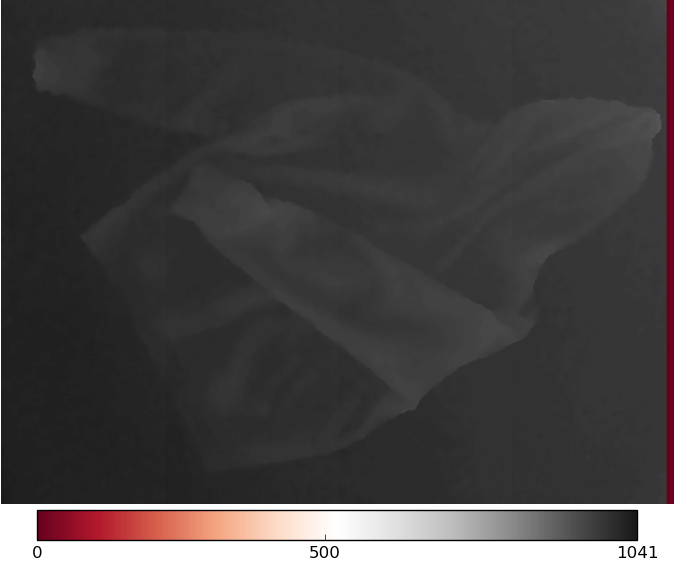
\includegraphics[width=\textwidth]
    	{figures/point-cloud-projection-2.png}
    	\caption{Depth Map}
	\end{subfigure}
    \caption[Comparison of the 3D point cloud with the Depth map obtained from its projection onto the table.]
    {Comparison of the 3D point cloud with the Depth map obtained from its projection onto the table. The colorbar beneath the second figure shows how depth from the camera (in mm) is mapped to the figure colors.}
    \label{fig:point_cloud_and_depth_image}
\end{figure}

The RGB values are also recorded for each depth image, obtaining an RGB-D image.


	\chapter{Conclusions and future work}
\label{conclusions_and_future_work}

\section{Conclusions}
\label{conclusions}
\section{Future Work}
\label{future_work}

\bibliographystyle{apacite}
\bibliography{library}
		
\end{document}